%% thesis.tex 2014/04/11
%
% Based on sample files of unknown authorship.
%
% The Current Maintainer of this work is Paul Vojta.

\documentclass{style/ucbthesis}
\usepackage[sorting=none, style=ieee]{biblatex}
\usepackage{style/variables}

\usepackage{amsmath}
\usepackage{amssymb}
\usepackage{amsfonts}
\usepackage{url}
\usepackage{hyperref}
\usepackage{graphicx}
\usepackage{float}
\usepackage{todonotes}
\usepackage{diagbox}
\usepackage{mathrsfs}
\usepackage[version=3]{mhchem}
\usepackage{algorithm}
\usepackage[noend]{algpseudocode}
\usepackage{varwidth}
\usepackage{parnotes}
\usepackage{graphicx}
\usepackage{tikz}
\usepackage{multirow}
\usepackage{tabularx}
\usepackage{booktabs}
\usepackage{siunitx}
\usepackage{enumitem}
\usepackage{wasysym}
\usepackage{pdflscape}
\usepackage{multicol}

% Tikz
\usepackage{tikz}
\usetikzlibrary{positioning,shapes,arrows,arrows.meta,snakes}
\tikzstyle{process} = [rectangle, text centered, draw=black,thick]
\tikzstyle{decision} = [diamond, text centered, draw=black,thick]
\tikzstyle{arrow} = [-{Stealth[scale=1.2]},rounded corners,thick]

% Captions
\usepackage[font=small,labelfont=bf]{caption}
\captionsetup{labelsep=period}

% Fonts
\usepackage{lettrine}% For drop caps at the start of each chapter
\usepackage[sc]{mathpazo}
\linespread{1.05}
\usepackage[T1]{fontenc}
% \renewcommand{\familydefault}{\sfdefault}
% \usepackage{palatino}
% \renewcommand{\rmdefault}{ppl} % rm
% \linespread{1.05}        % Palatino needs more leading
% % \usepackage{euler} % math
% \normalfont
% \usepackage[T1]{fontenc}

% List of acronyms
\usepackage[toc, acronym, nopostdot, nonumberlist, nogroupskip]{glossaries}
\makeglossaries
\usepackage{style/abbreviations}

% Table of content depth
\setcounter{tocdepth}{5}

% Section numbering depth
\setcounter{secnumdepth}{5}

% Parnotes config
\renewcommand*\parnoteintercmd[1]{,\,}

% Figure borders
\setlength{\fboxsep}{0pt}
\setlength{\fboxrule}{0.25pt}

% Error function
\DeclareMathOperator\erf{erf}

% To compile this file, run "latex thesis", then "biber thesis"
% (or "bibtex thesis", if the output from latex asks for that instead),
% and then "latex thesis" (without the quotes in each case).

% Double spacing, if you want it.  Do not use for the final copy.
% \def\dsp{\def\baselinestretch{2.0}\large\normalsize}
% \dsp

% If the Grad. Division insists that the first paragraph of a section
% be indented (like the others), then include this line:
% \usepackage{indentfirst}

\bibliography{ref/references}

\hyphenation{mar-gin-al-ia}
\hyphenation{bra-va-do}

\newcommand*{\MyPath}{.}%

\begin{document}

\title{\thesistitle}
\author{\thesisauthor}
\degreesemester{\thesisdegreesemester}
\degreeyear{\thesisdegreeyear}
\degree{\thesisdegree}
\chair{\thesischair}
\othermembers{\thesiscommittee}
\numberofmembers{\thesiscommitteenum}
% Previous degrees are no longer to be listed on the title page.
% \prevdegrees{B.A. (University of Northern South Dakota at Hoople) 1978 \\
%   M.S. (Ed's School of Quantum Mechanics and Muffler Repair) 1989}
\field{\thesisfield}
% Designated Emphasis -- this is optional, and rare
% \emphasis{Colloidal Telemetry}
% This is optional, and rare
% \jointinstitution{University of Western Maryland}
% This is optional
\campus{\thesiscampus}

% For a masters thesis, replace the above \documentclass line with
% \documentclass[masters]{ucbthesis}
% This affects the title and approval pages, which by default calls this
% document a "dissertation", not a "thesis".

\maketitle

\title{\thesistitle}
\author{\thesisauthor}
\chair{\thesischair}
\othermembers{\thesiscommittee}
\numberofmembers{\thesiscommitteenum}
\campus{\thesiscampus}

\approvalpage
\title{\thesistitle}
\author{\thesisauthor}
\degreeyear{\thesisdegreeyear}

\copyrightpage
\title{\thesistitle}
\author{\thesisauthor}
\degreesemester{\thesisdegreesemester}
\degreeyear{\thesisdegreeyear}
\degree{\thesisdegree}
\chair{\thesischair}
\field{\thesisfield}
\campus{\thesiscampus}

\begin{abstract}

Text goes here.

\end{abstract}


\begin{frontmatter}
	\begin{dedication}

\null\vfil
\begin{center}

To someone\\\vspace{12pt}

Text goes here.

\end{center}
\vfil\null

\end{dedication}
	\tableofcontents
\clearpage
\listoffigures
\clearpage
\listoftables
\clearpage
\listofacronyms

	\begin{acknowledgements}

Text.

\end{acknowledgements}

\end{frontmatter}

%\pagestyle{headings}

\renewcommand*{\MyPath}{./Chapters/ch6}
\renewcommand{\thechapter}{6}
\graphicspath{{\MyPath/}}

\chapter{Title} \label{sec:title}
Text.


\section{Title} \label{sec:section}
Text. \acrfull{asap}.


\section{Title} \label{sec:section}
Text.
%
\begin{figure}[H]
    \hypertarget{fig1}{}
    \centering
    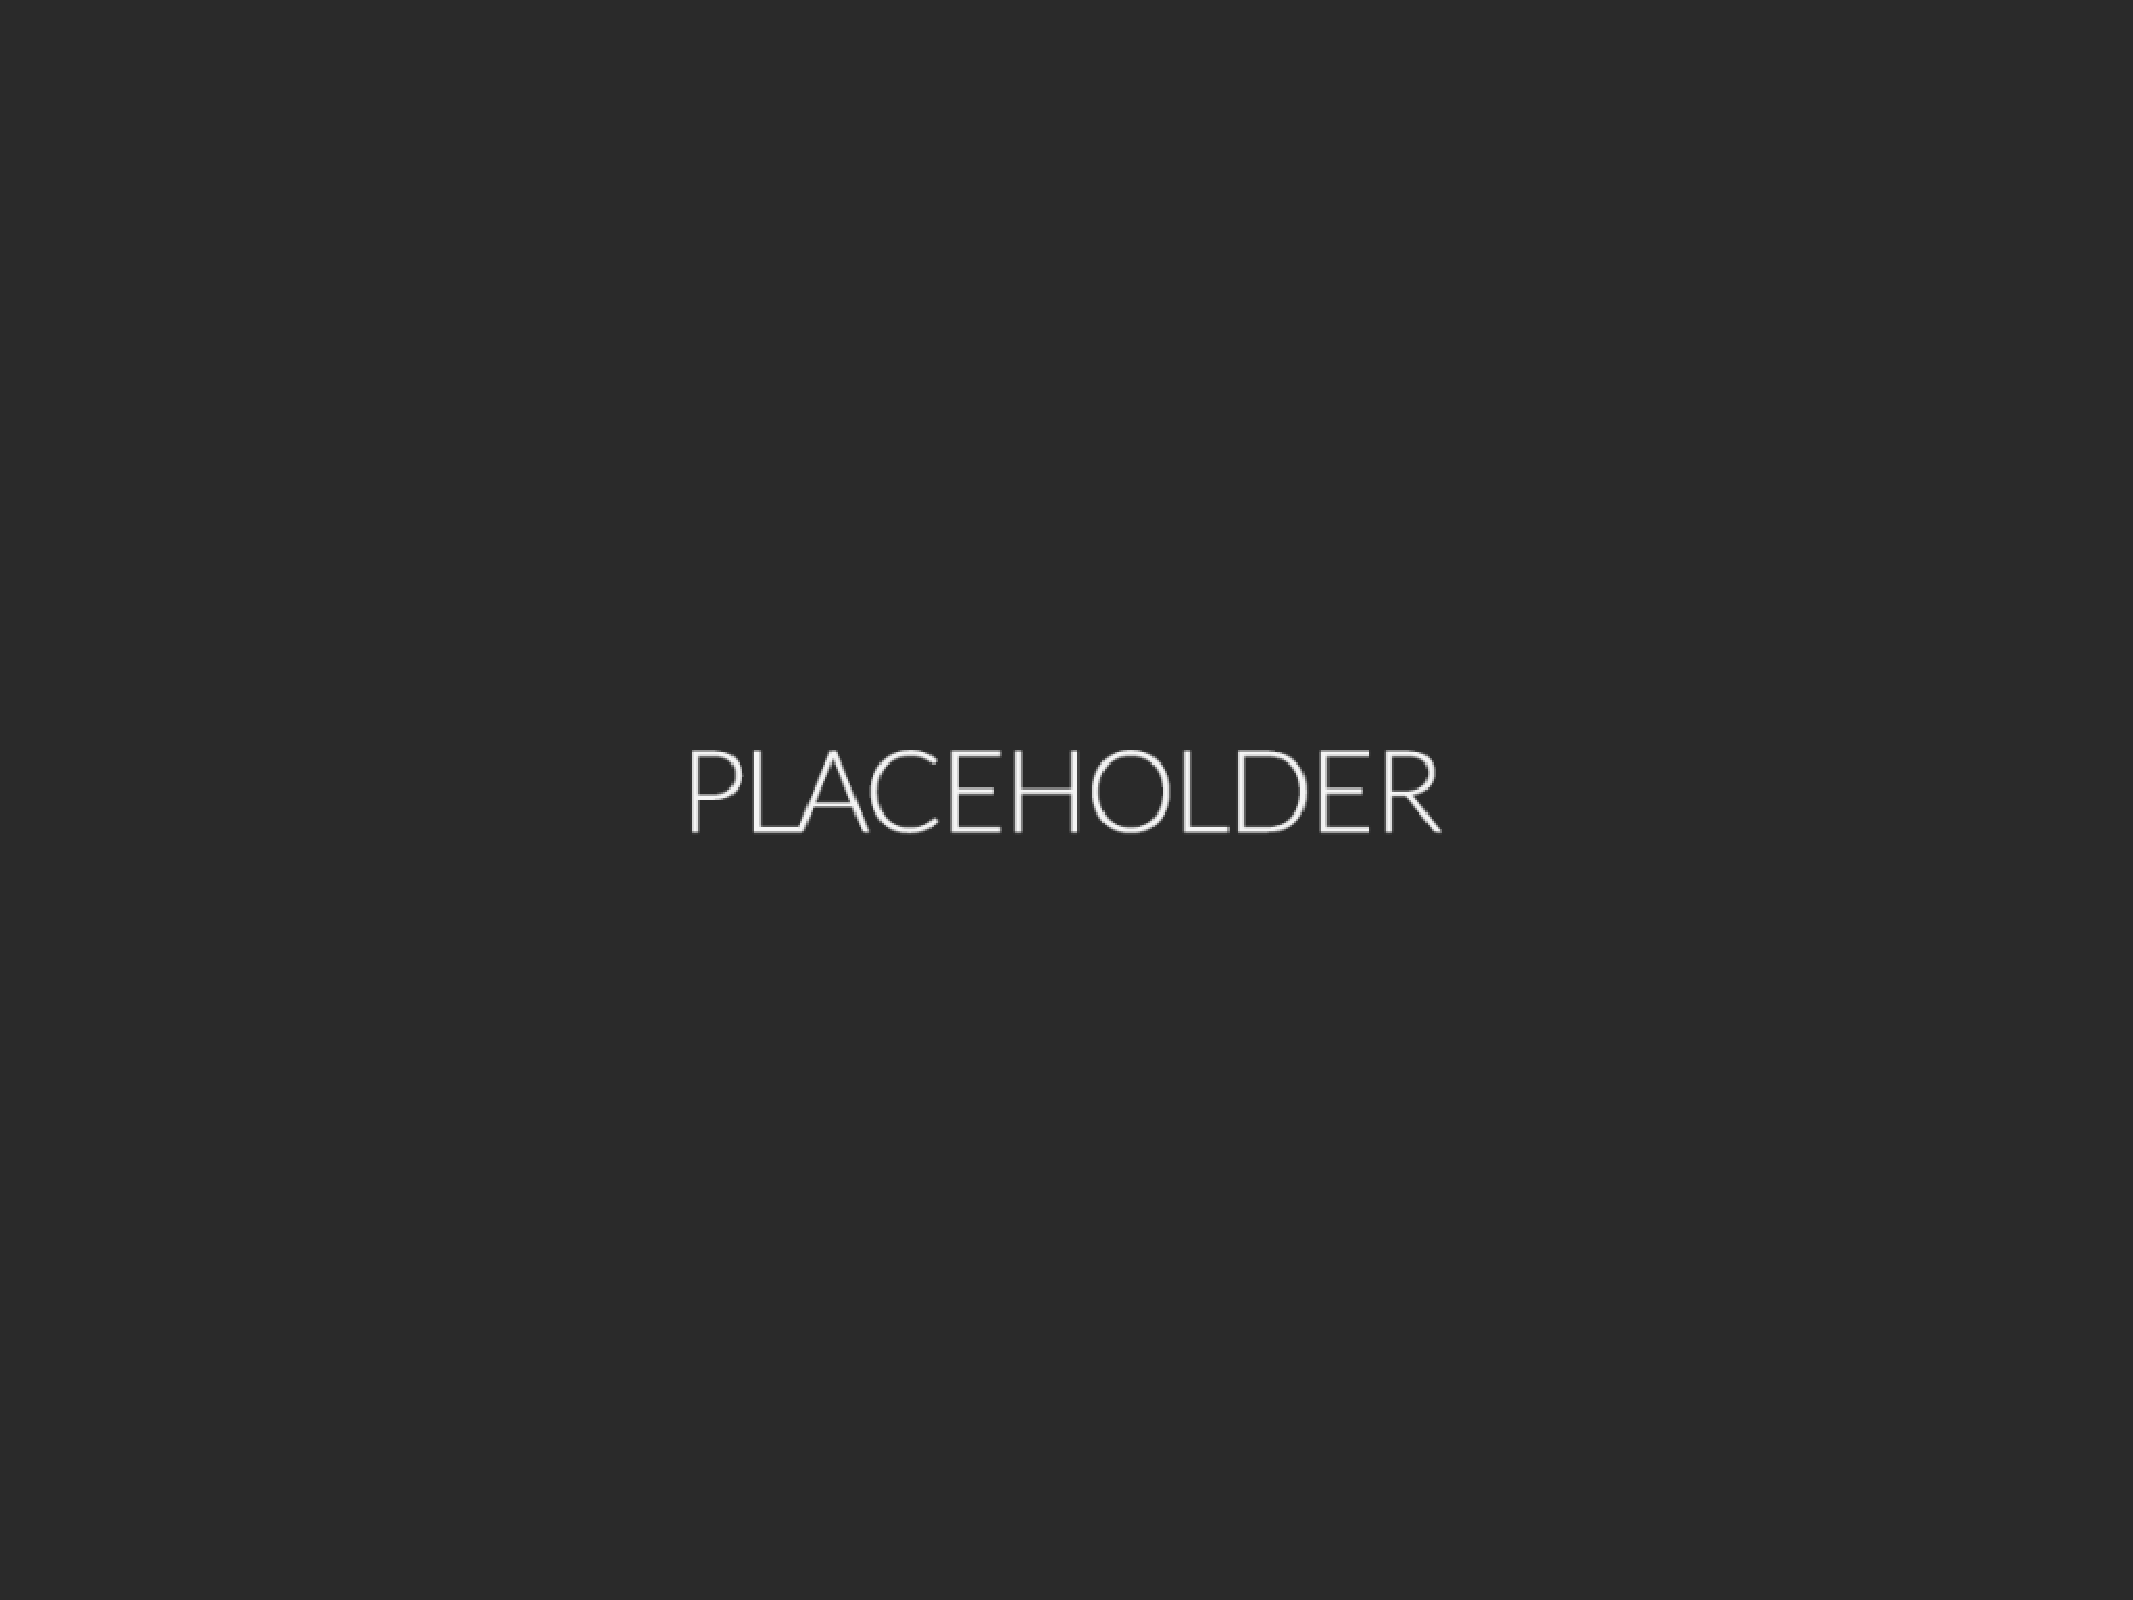
\includegraphics[width=0.5\columnwidth]{fig/placeholder.pdf}
    \caption{Caption goes here.}
\end{figure}
%
\begin{figure}[H]
    \hypertarget{fig2}{}
    \centering
    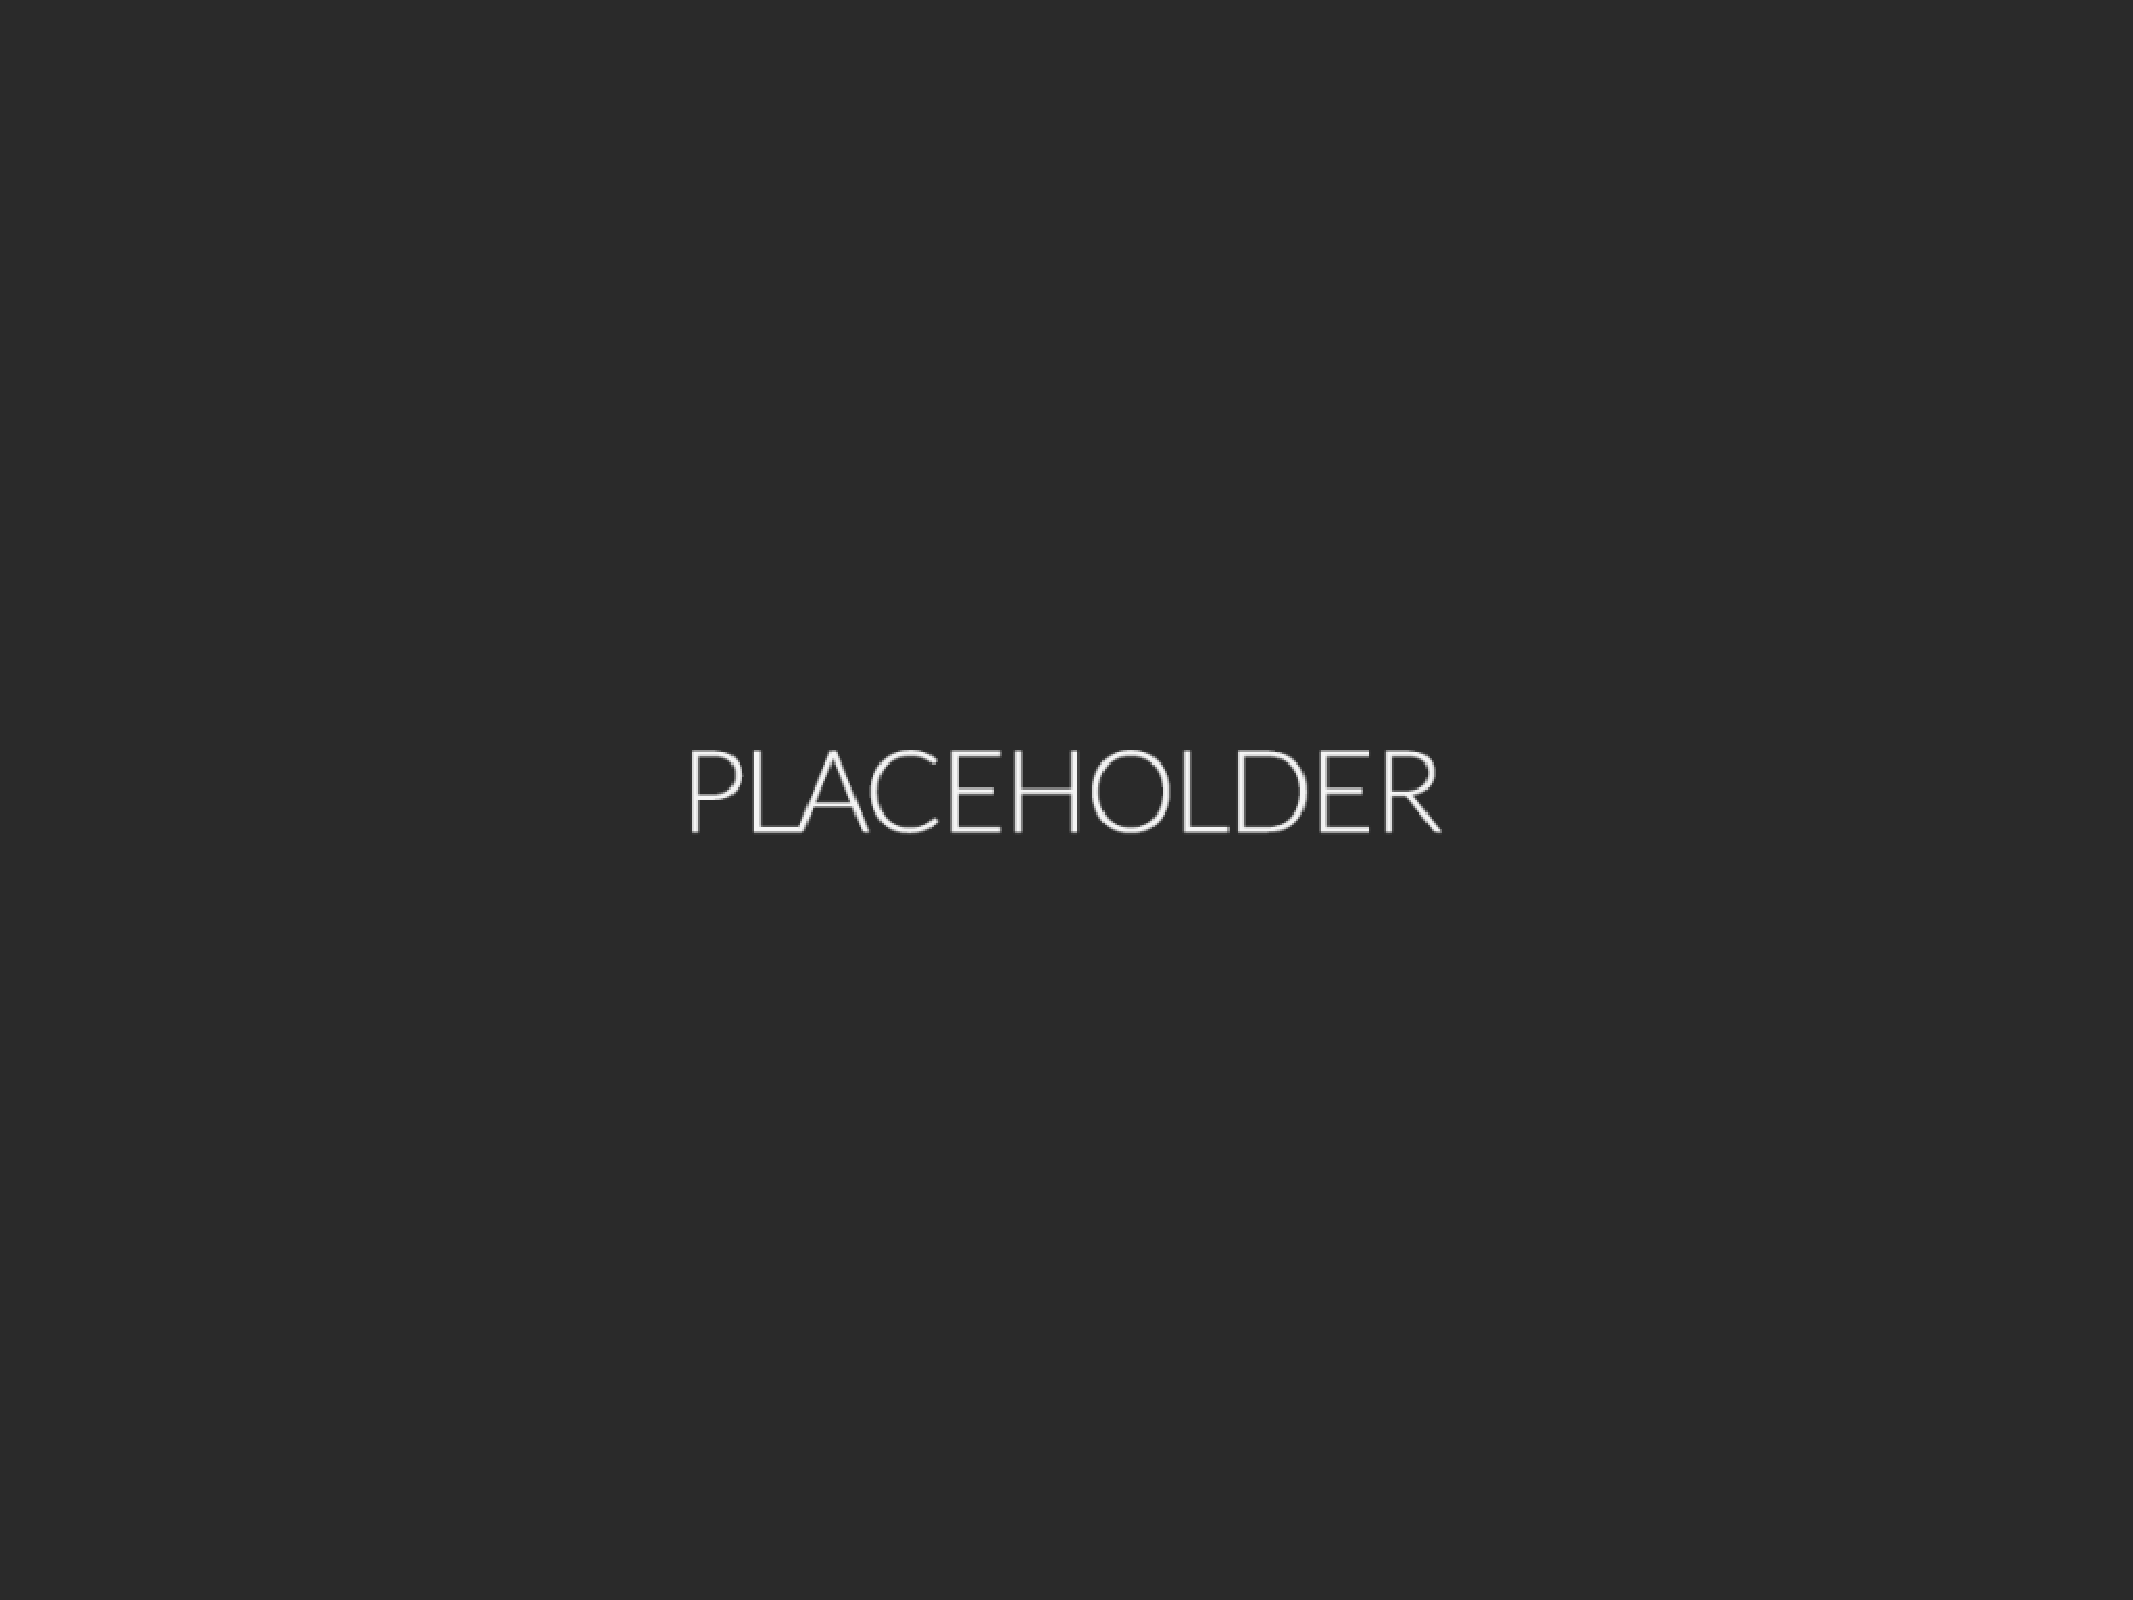
\includegraphics[width=0.5\columnwidth]{fig/placeholder.pdf}
    \caption{Caption goes here.}
\end{figure}


\renewcommand*{\MyPath}{./Chapters/ch6}
\renewcommand{\thechapter}{6}
\graphicspath{{\MyPath/}}

\chapter{Title} \label{sec:title}
Text.


\section{Title} \label{sec:section}
Text. \acrfull{asap}.


\section{Title} \label{sec:section}
Text.
%
\begin{figure}[H]
    \hypertarget{fig1}{}
    \centering
    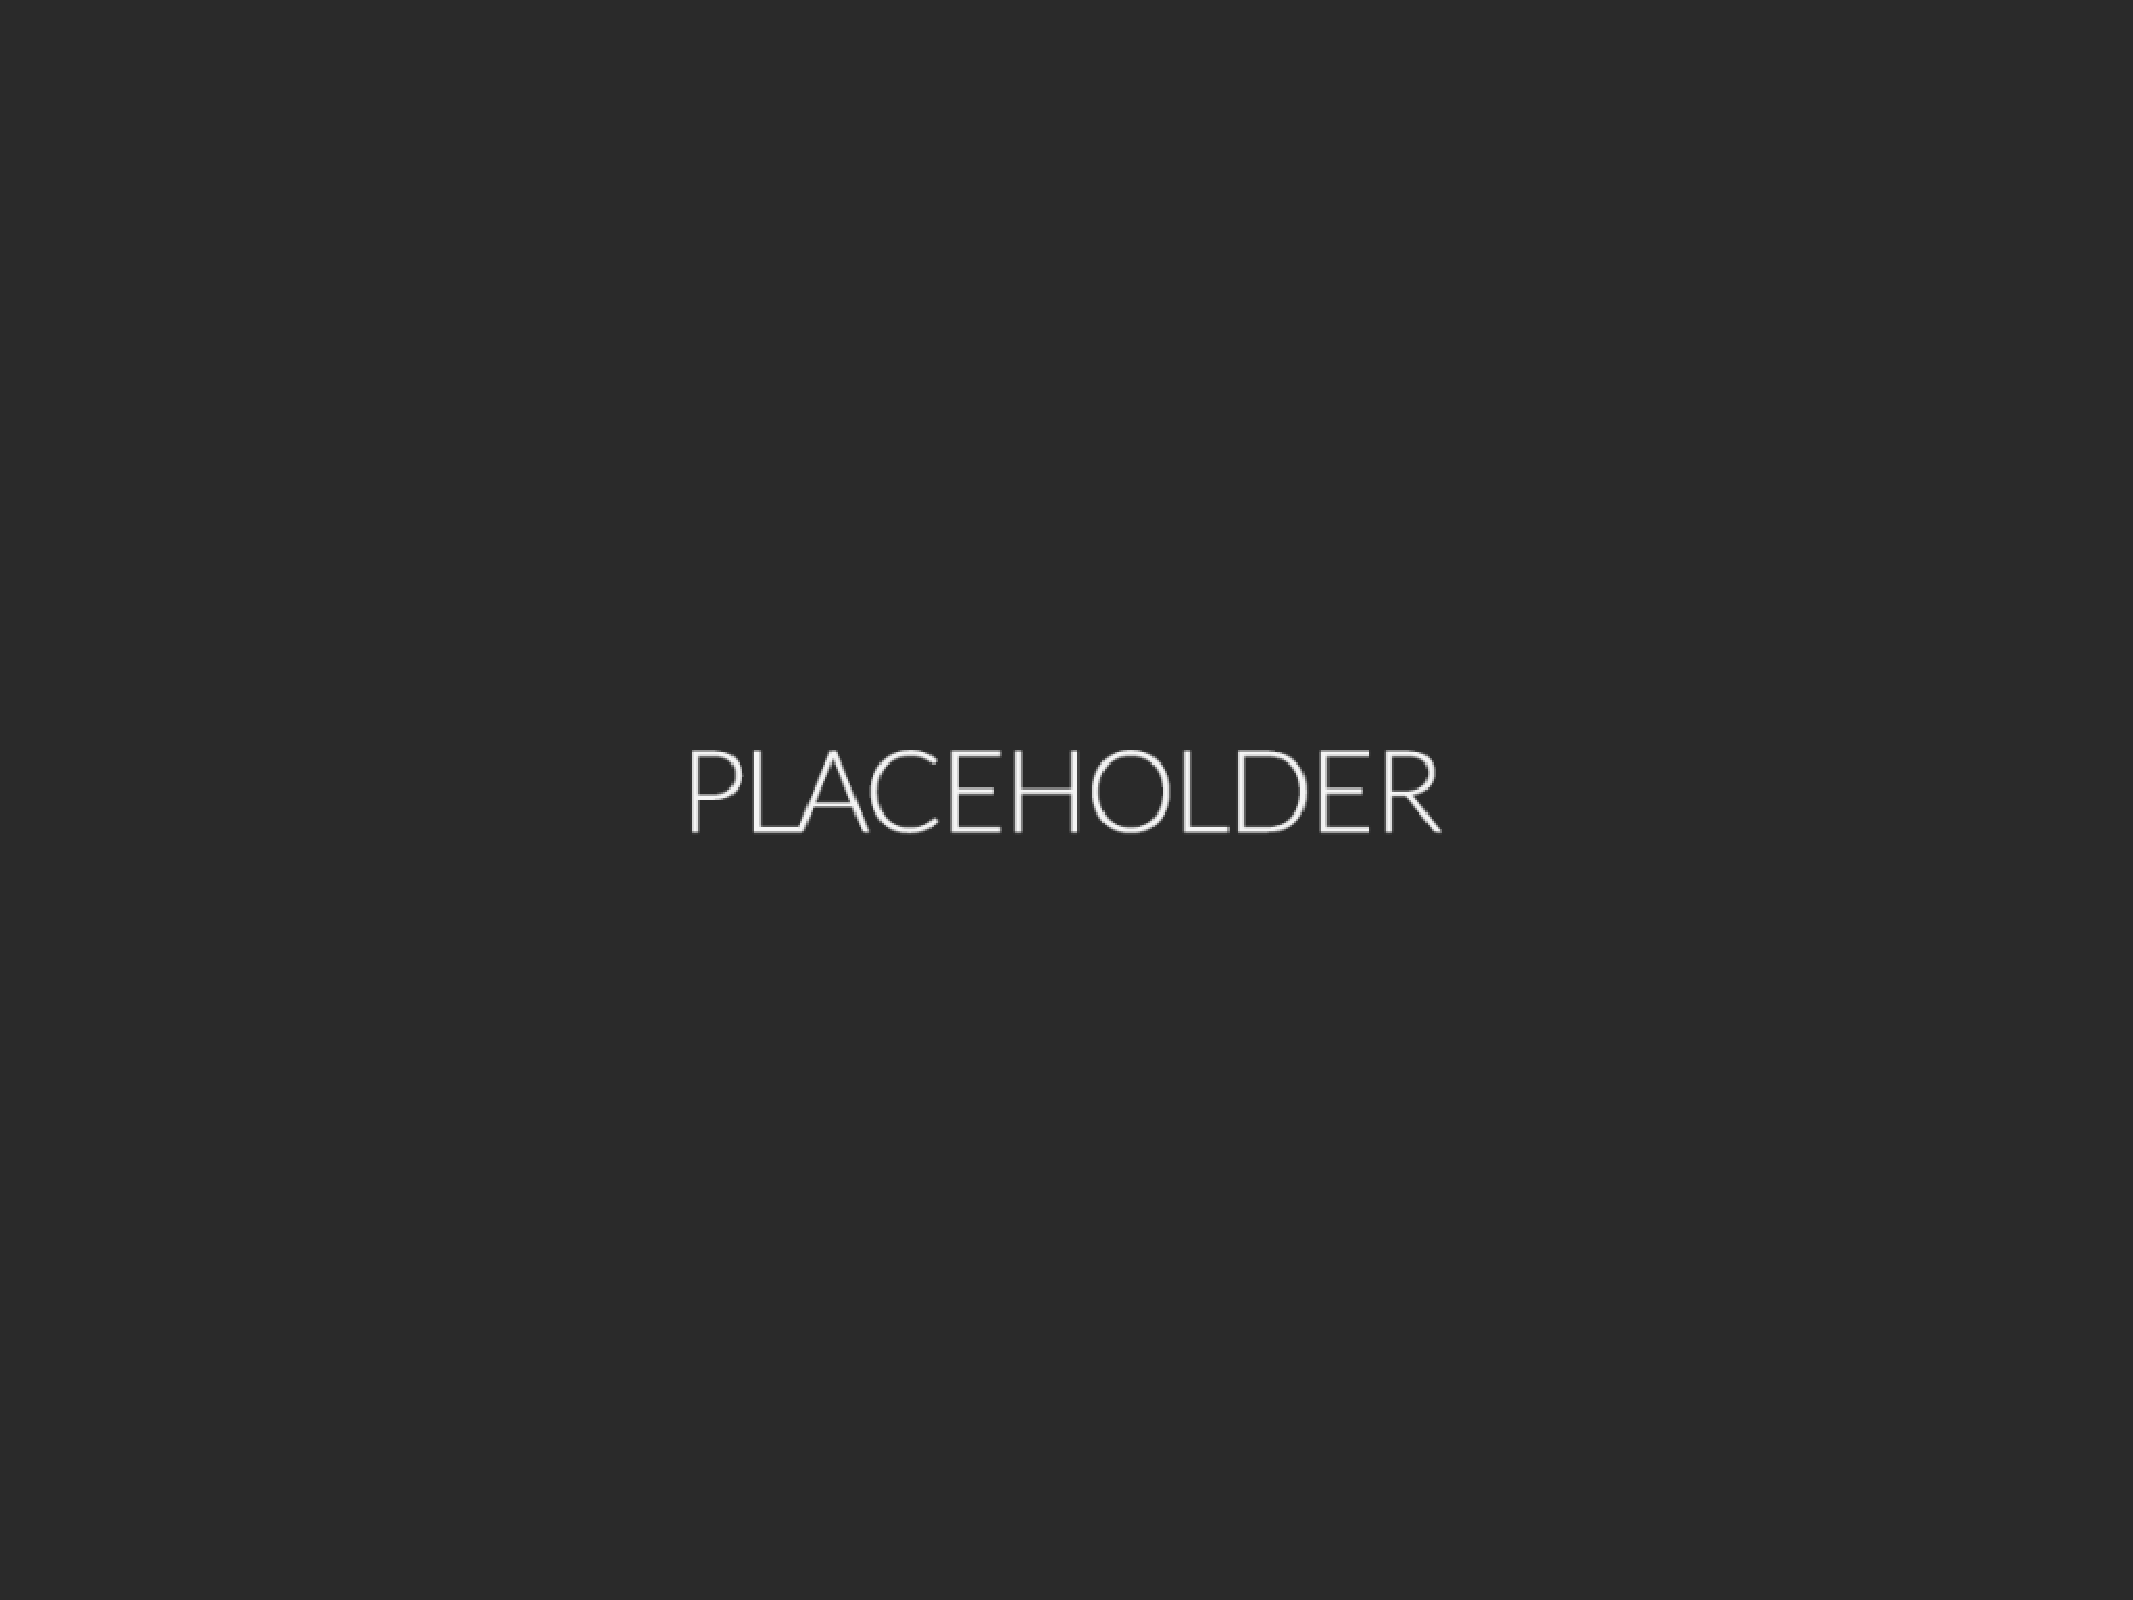
\includegraphics[width=0.5\columnwidth]{fig/placeholder.pdf}
    \caption{Caption goes here.}
\end{figure}
%
\begin{figure}[H]
    \hypertarget{fig2}{}
    \centering
    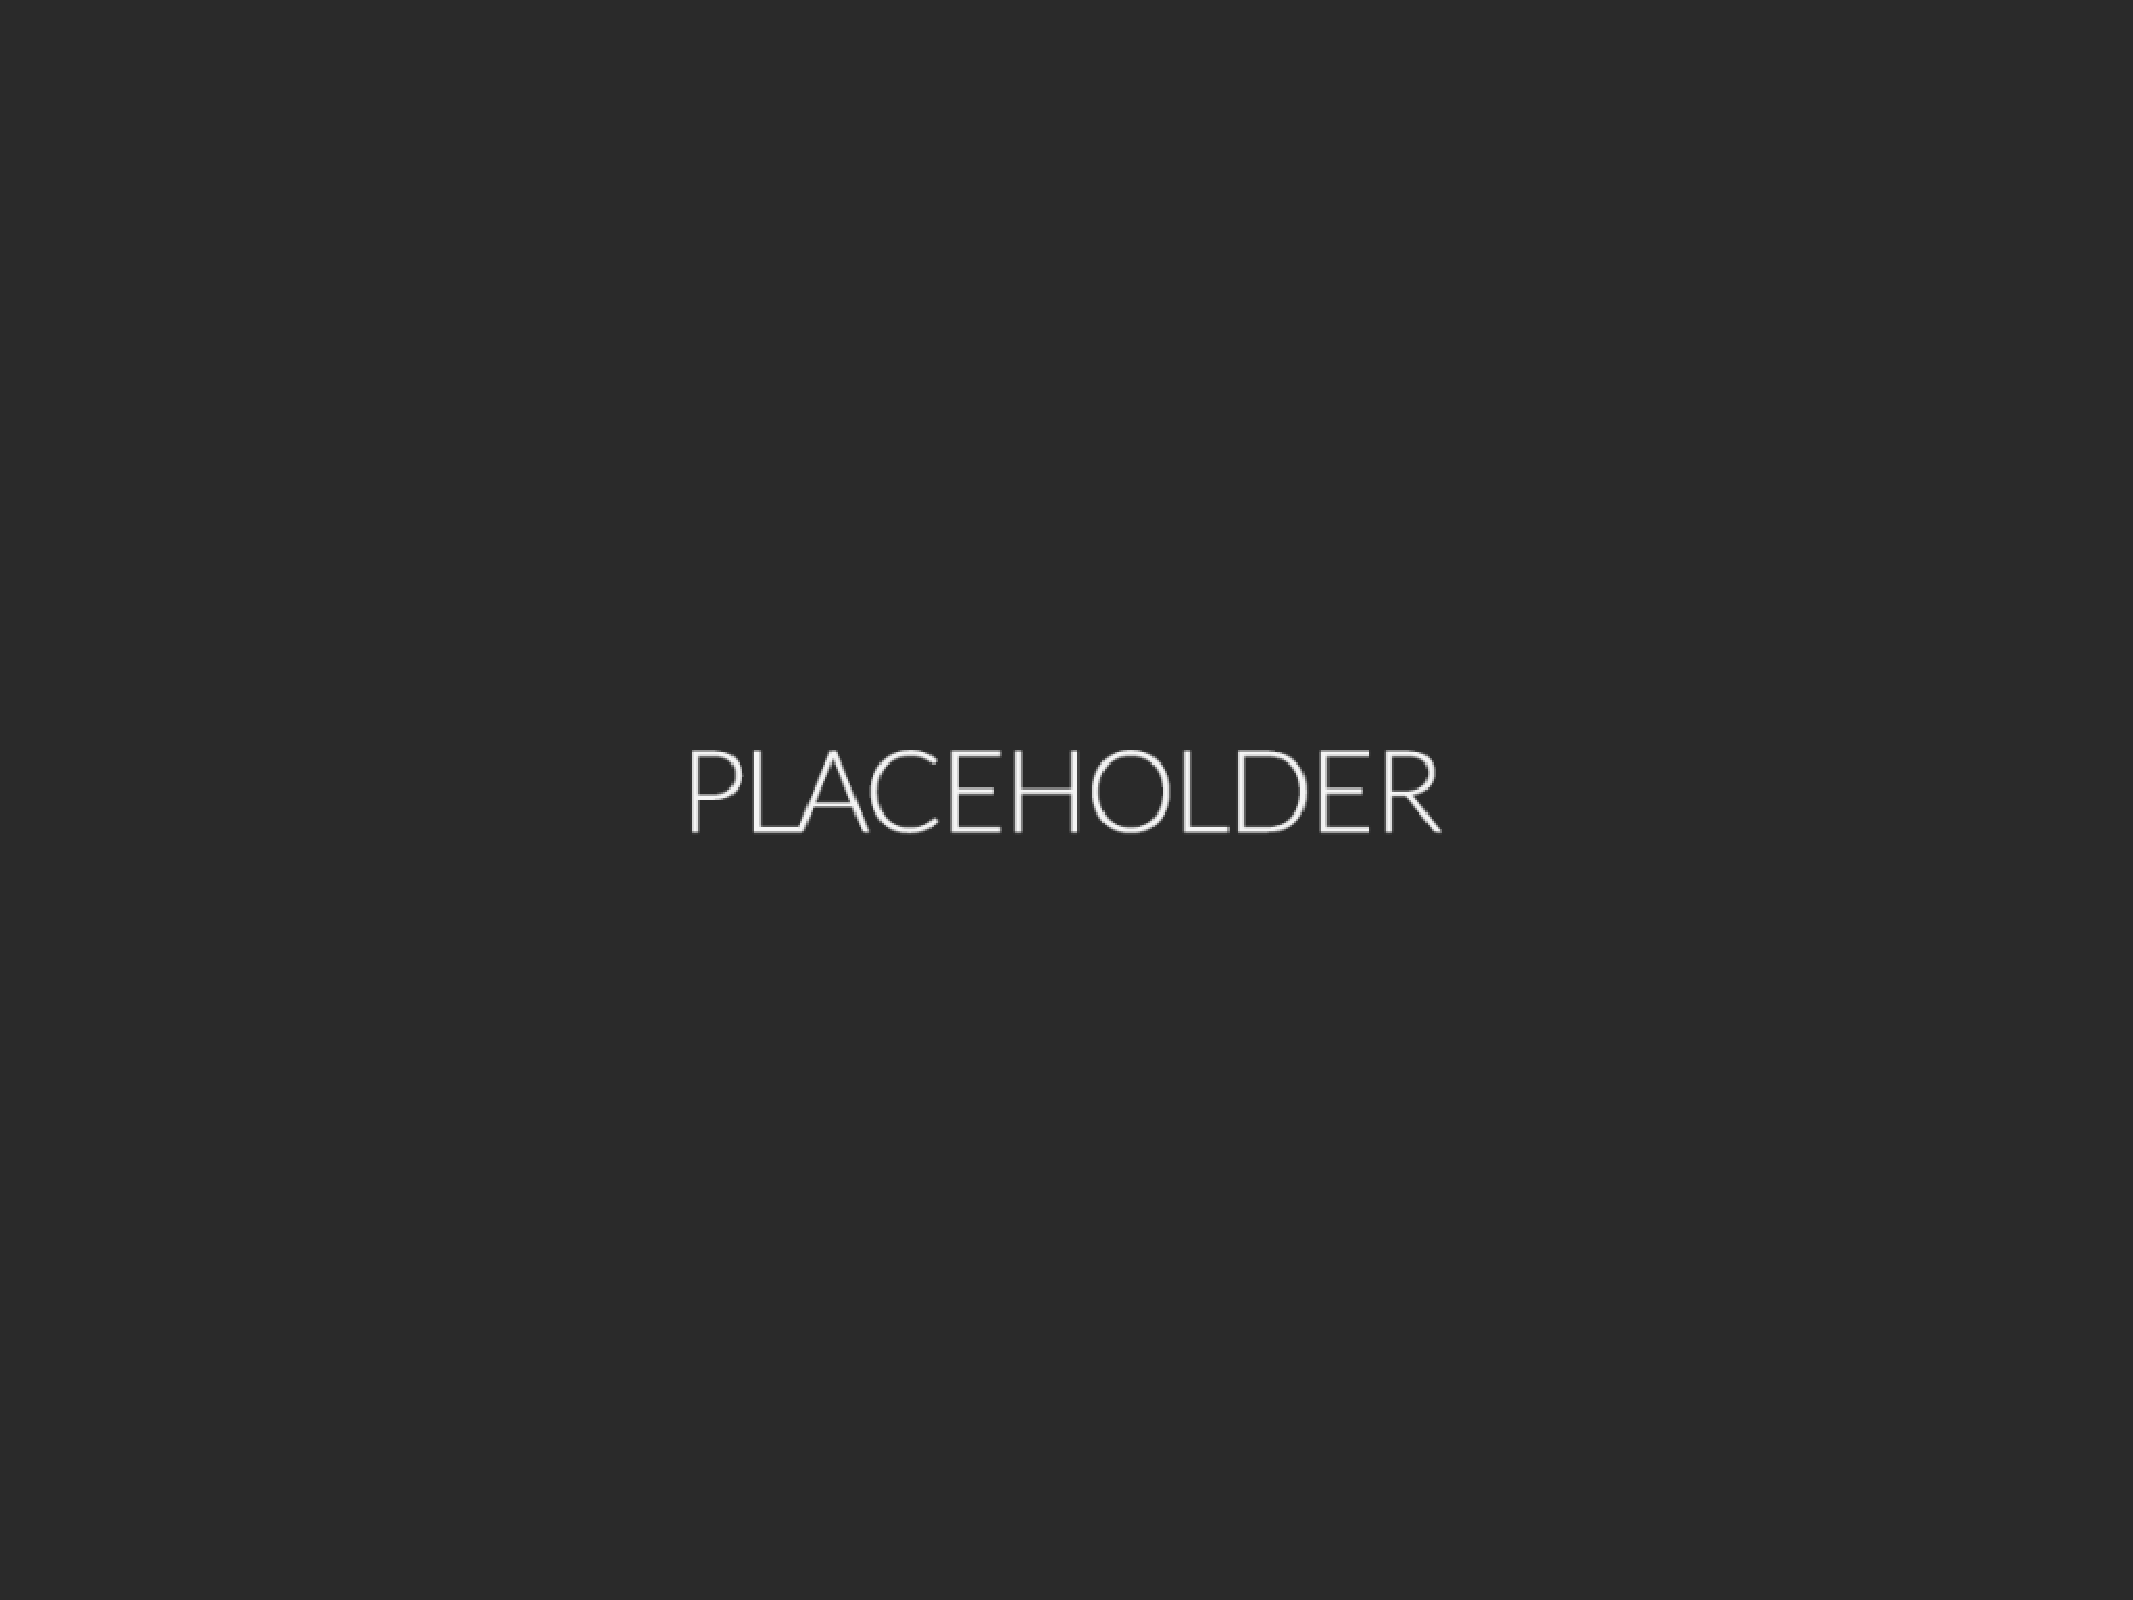
\includegraphics[width=0.5\columnwidth]{fig/placeholder.pdf}
    \caption{Caption goes here.}
\end{figure}


\renewcommand*{\MyPath}{./Chapters/ch6}
\renewcommand{\thechapter}{6}
\graphicspath{{\MyPath/}}

\chapter{Title} \label{sec:title}
Text.


\section{Title} \label{sec:section}
Text. \acrfull{asap}.


\section{Title} \label{sec:section}
Text.
%
\begin{figure}[H]
    \hypertarget{fig1}{}
    \centering
    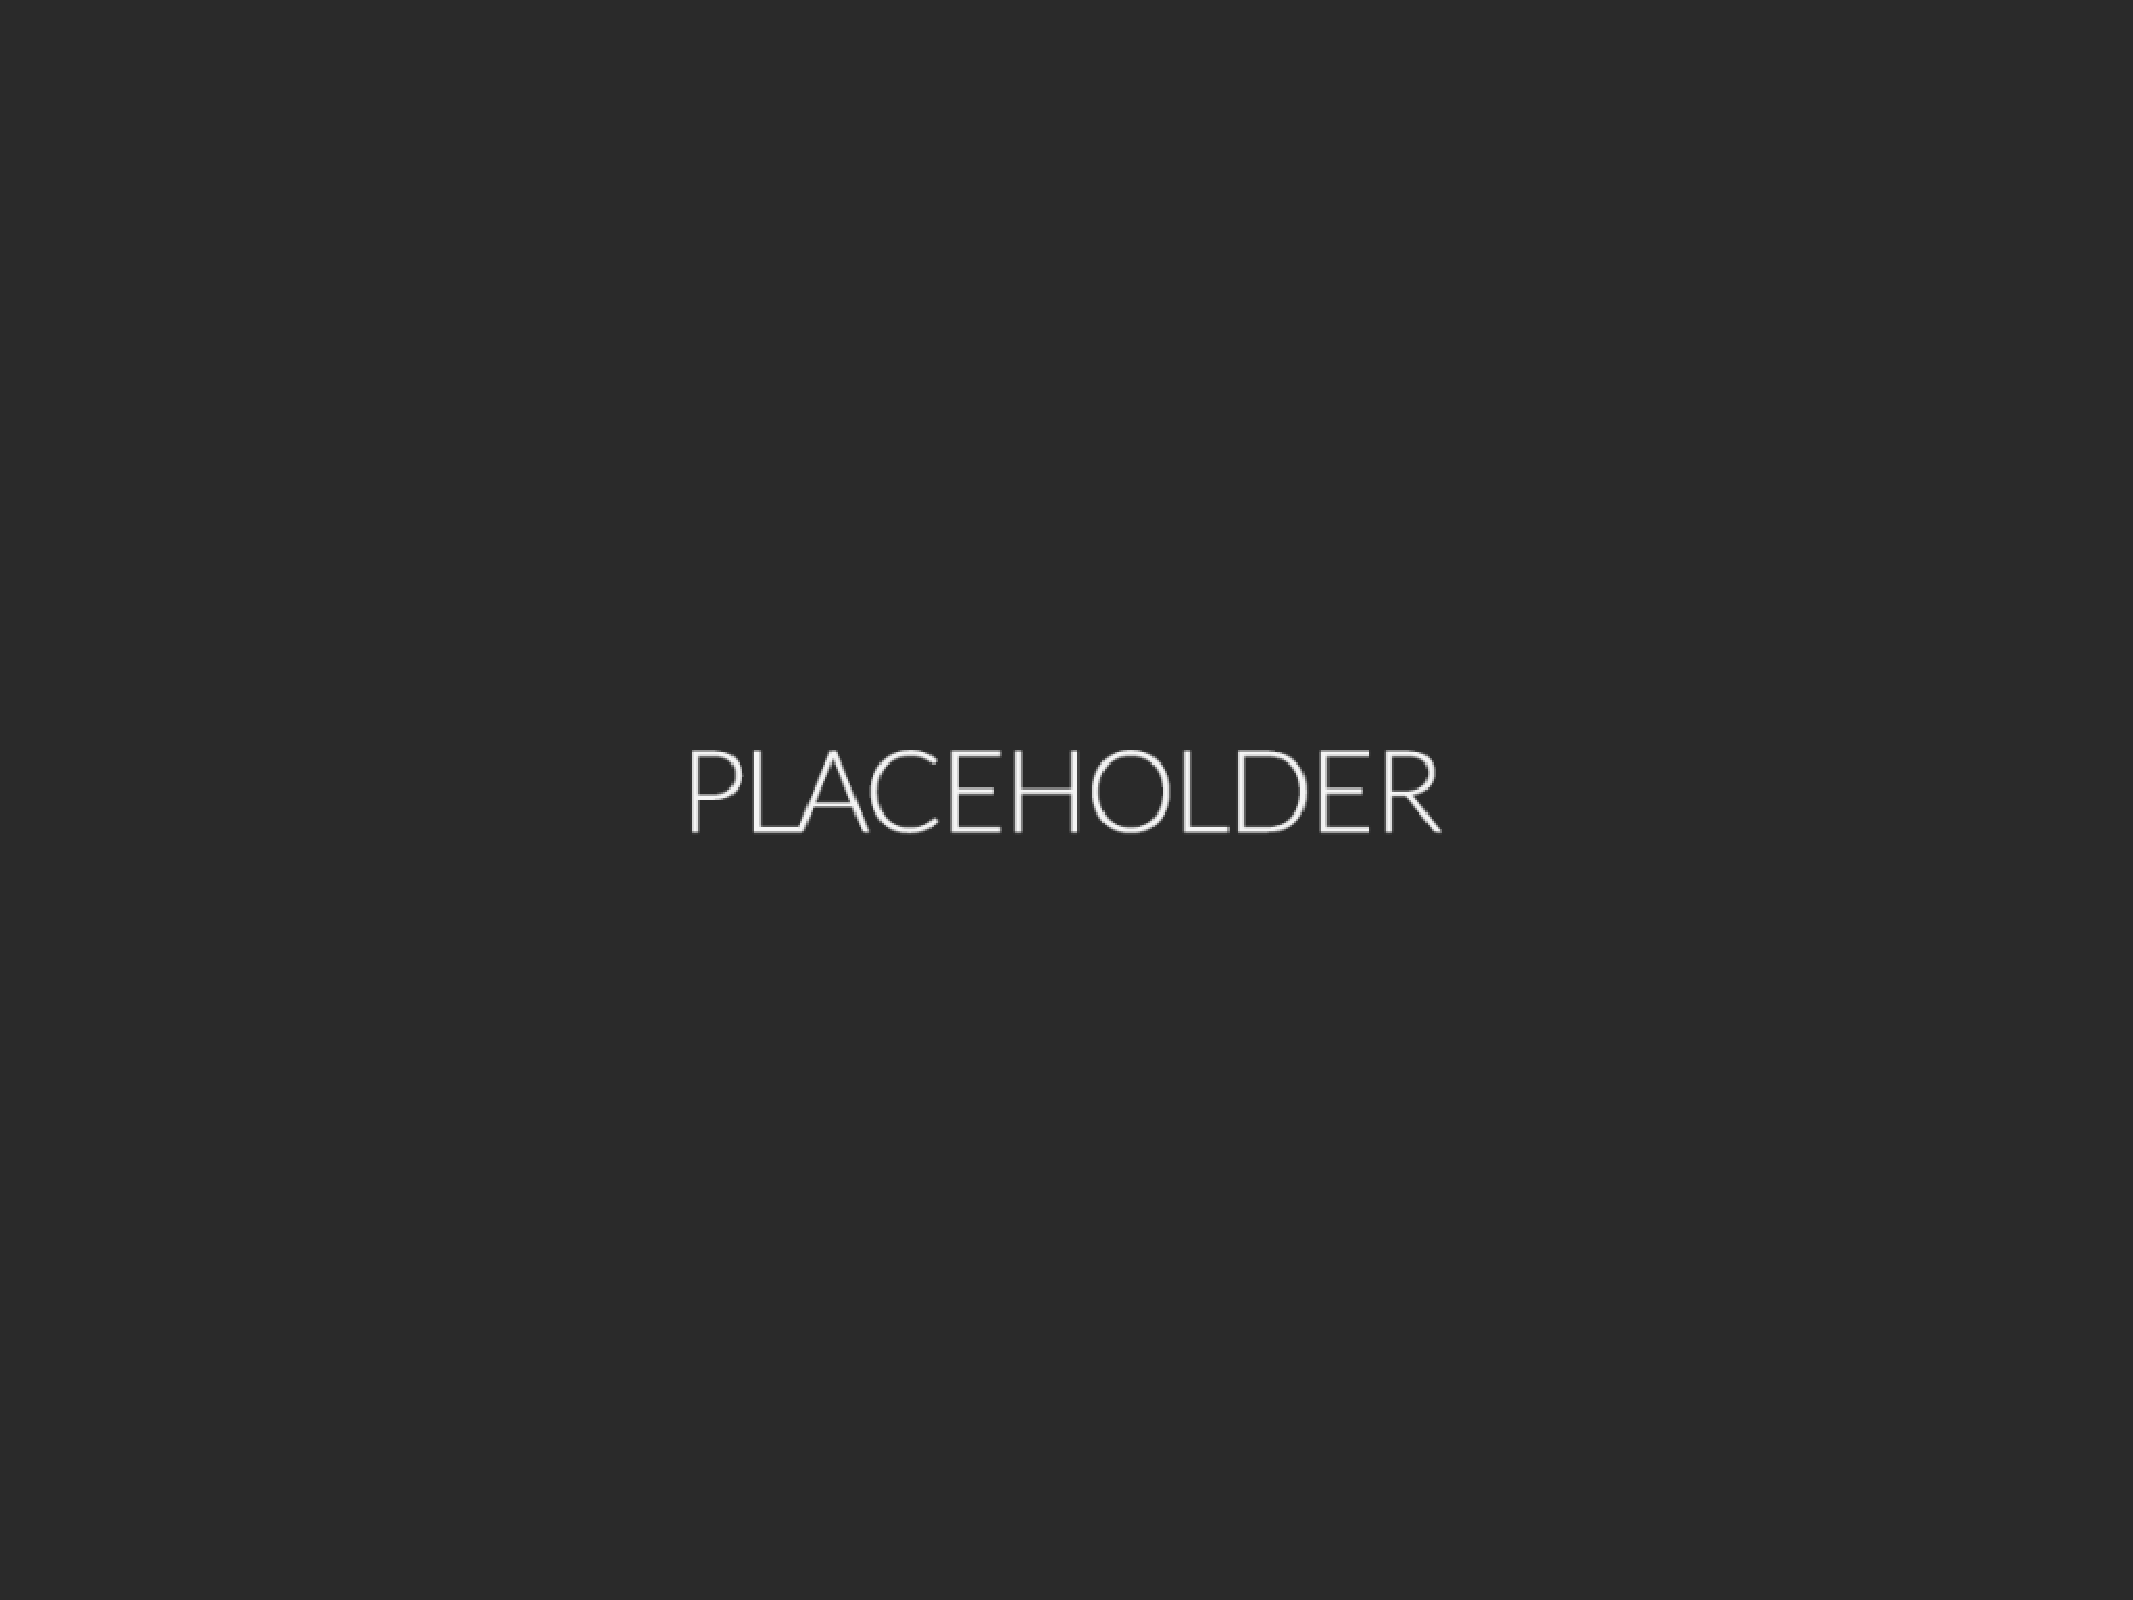
\includegraphics[width=0.5\columnwidth]{fig/placeholder.pdf}
    \caption{Caption goes here.}
\end{figure}
%
\begin{figure}[H]
    \hypertarget{fig2}{}
    \centering
    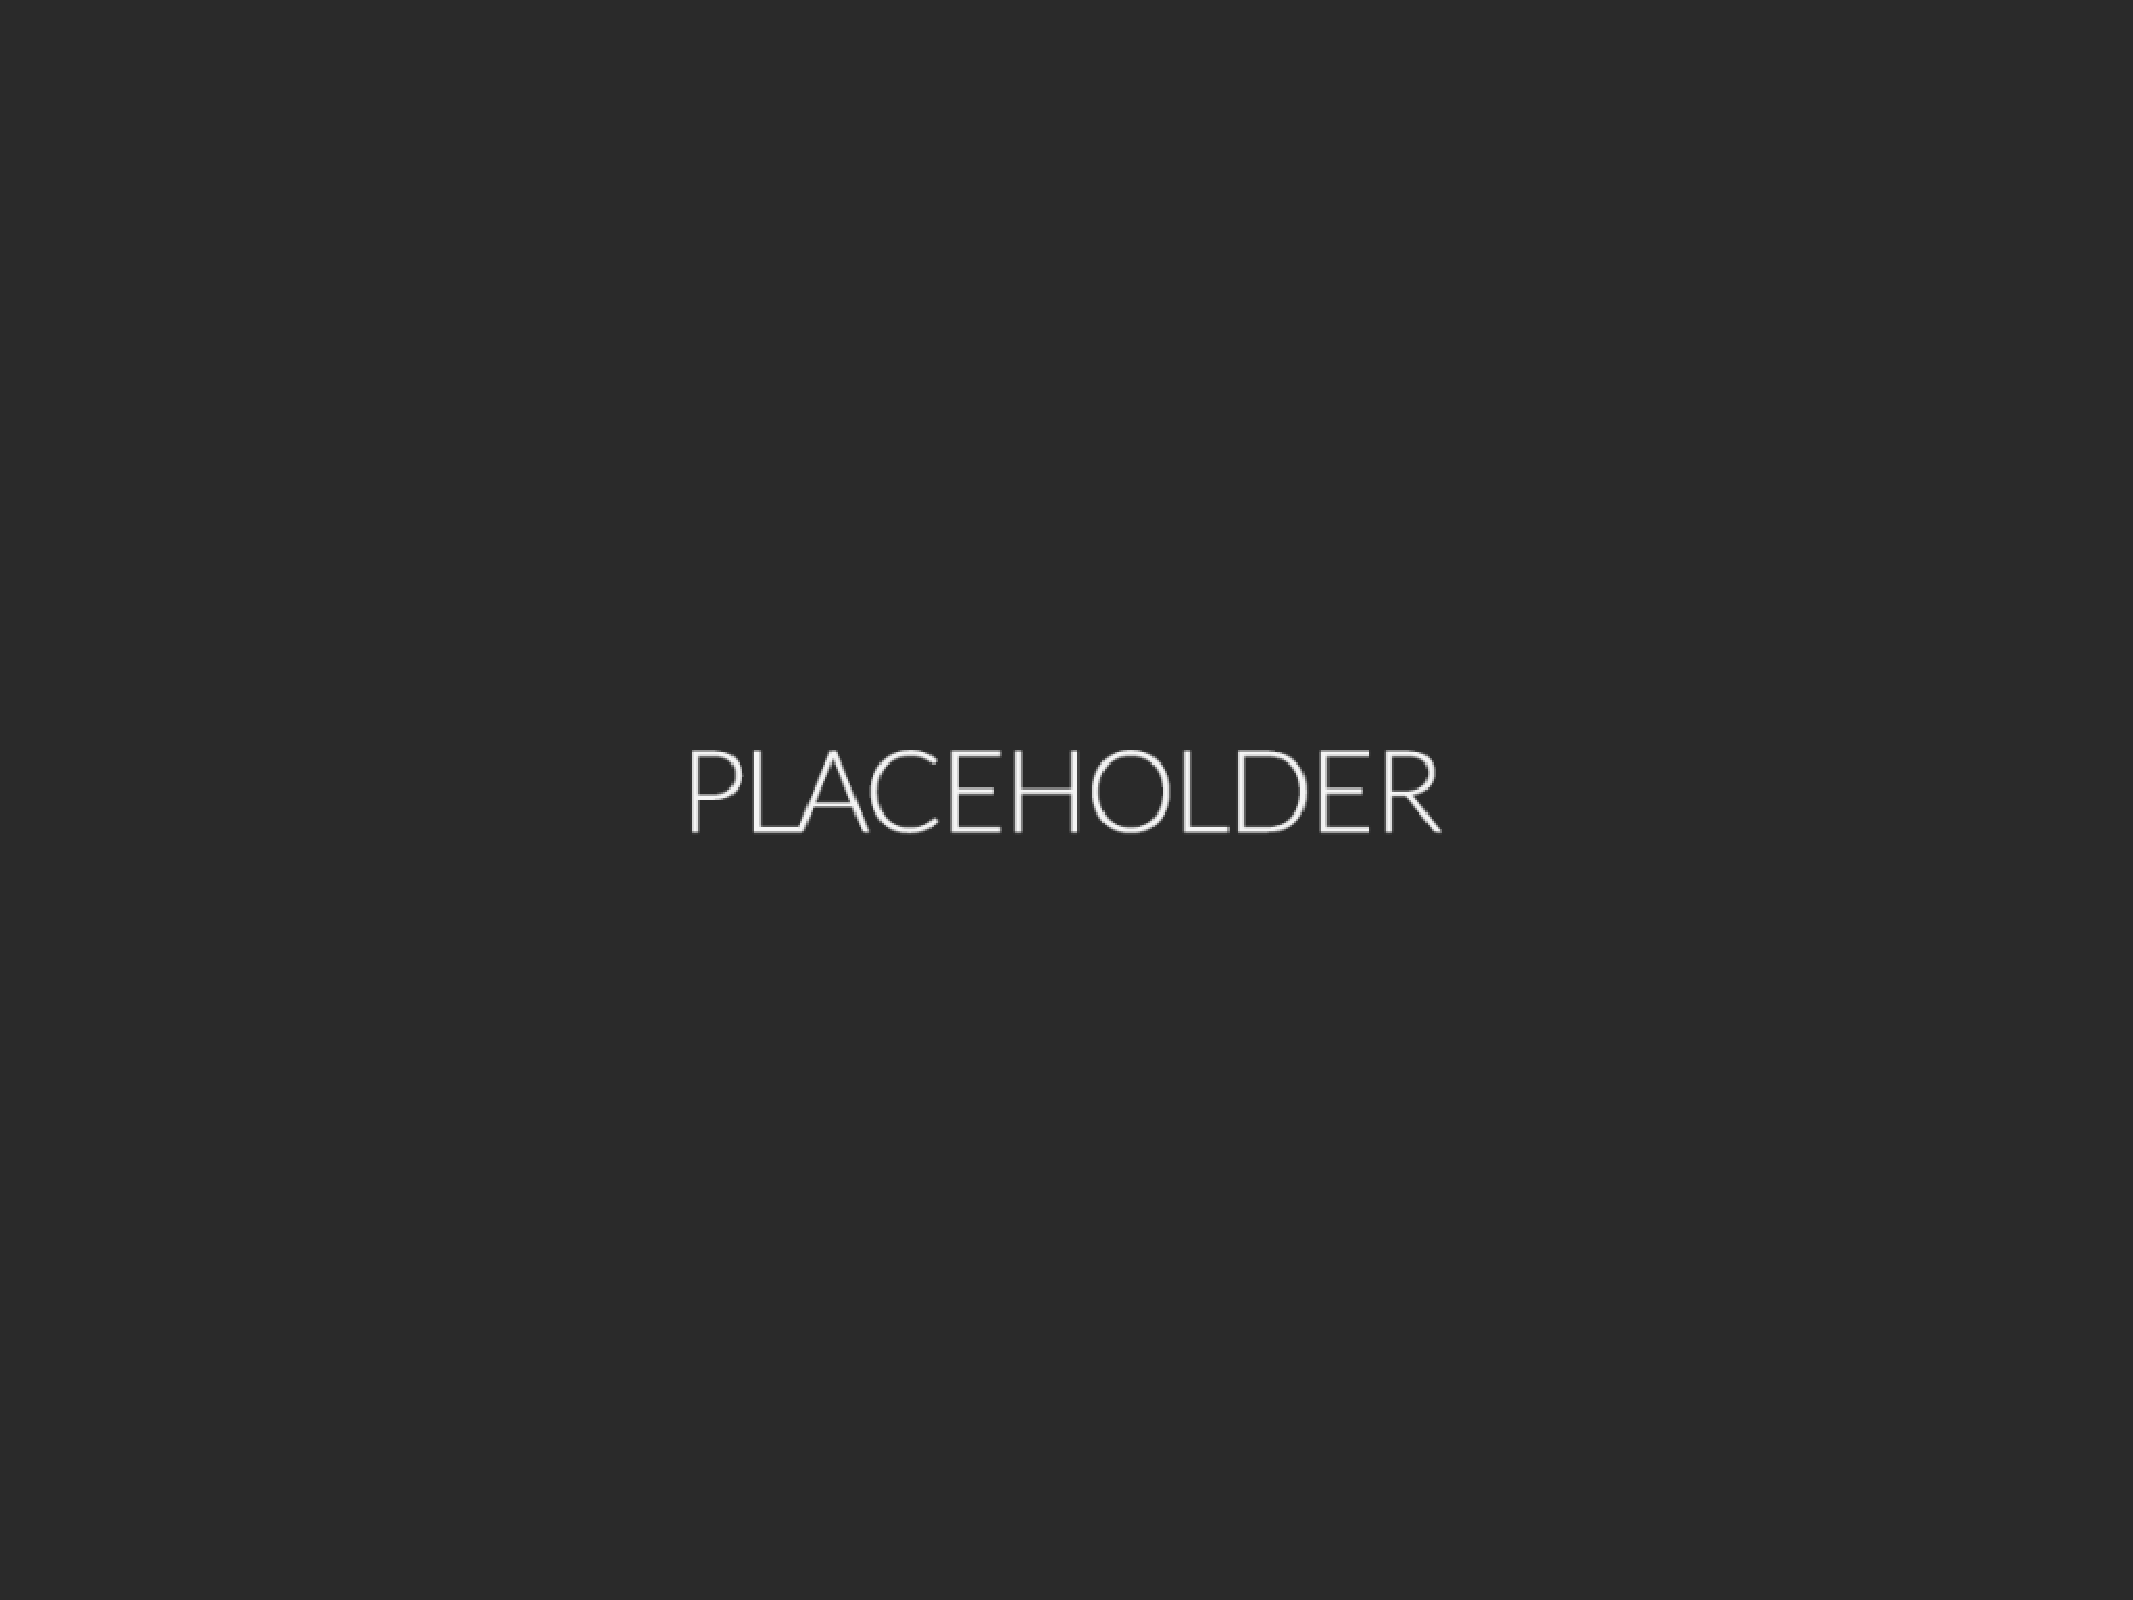
\includegraphics[width=0.5\columnwidth]{fig/placeholder.pdf}
    \caption{Caption goes here.}
\end{figure}


\renewcommand*{\MyPath}{./Chapters/ch6}
\renewcommand{\thechapter}{6}
\graphicspath{{\MyPath/}}

\chapter{Title} \label{sec:title}
Text.


\section{Title} \label{sec:section}
Text. \acrfull{asap}.


\section{Title} \label{sec:section}
Text.
%
\begin{figure}[H]
    \hypertarget{fig1}{}
    \centering
    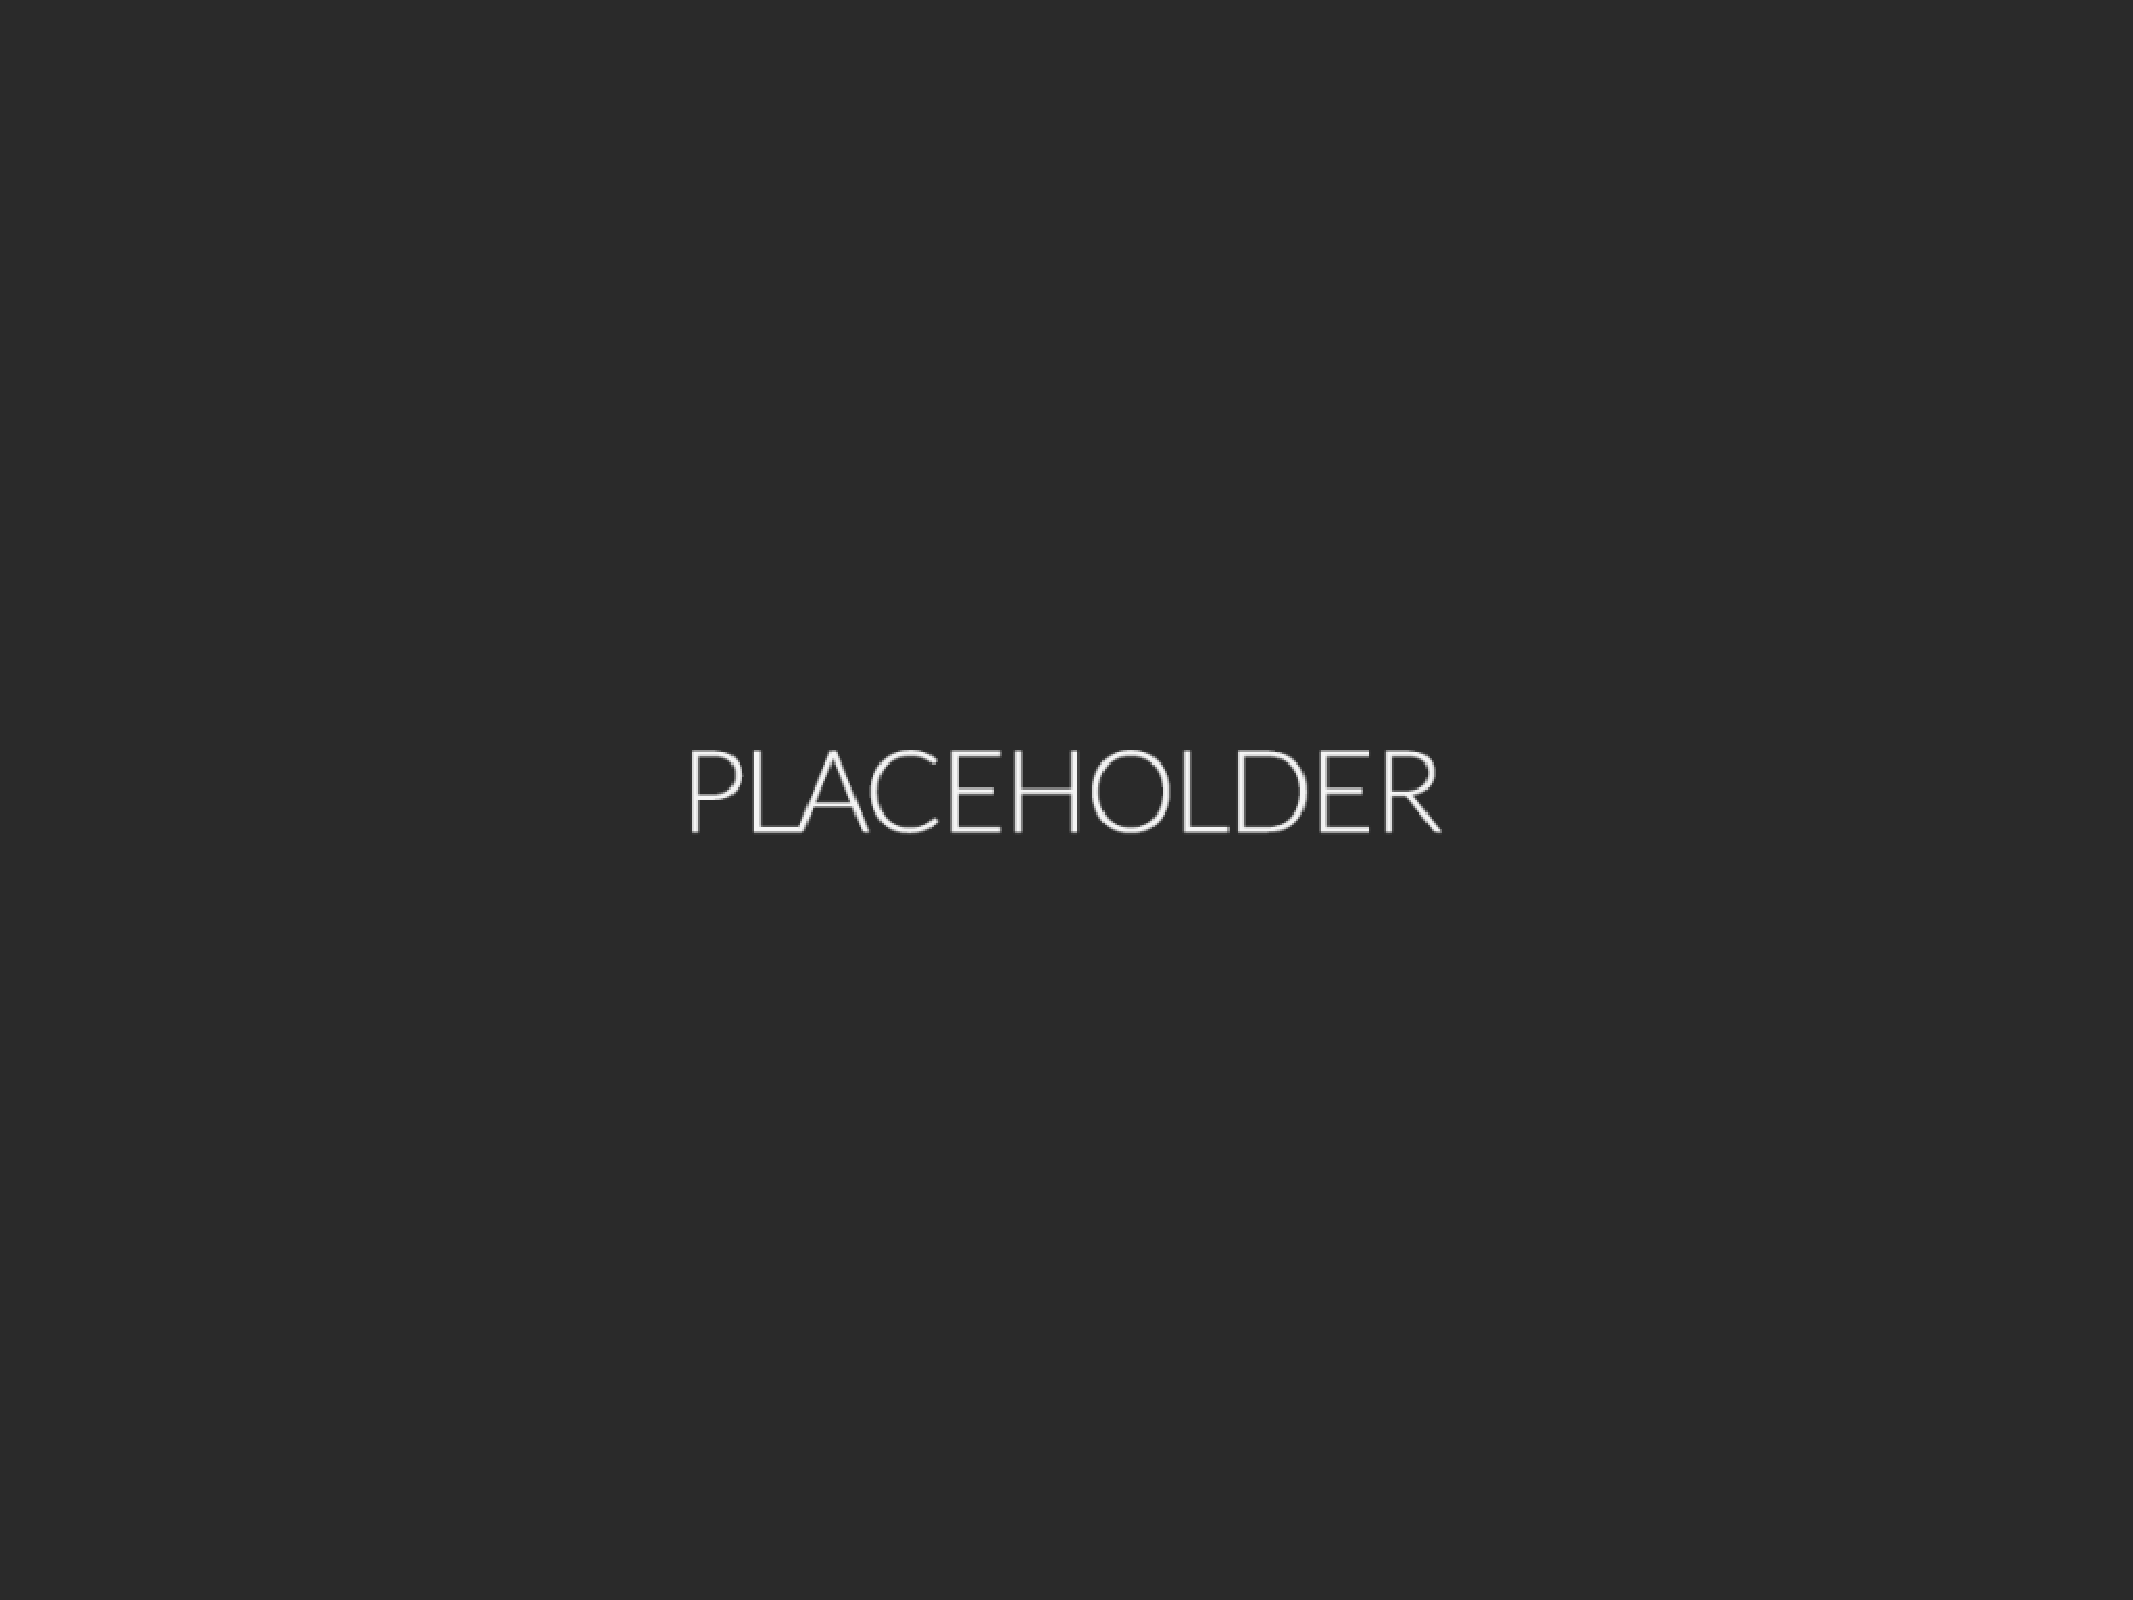
\includegraphics[width=0.5\columnwidth]{fig/placeholder.pdf}
    \caption{Caption goes here.}
\end{figure}
%
\begin{figure}[H]
    \hypertarget{fig2}{}
    \centering
    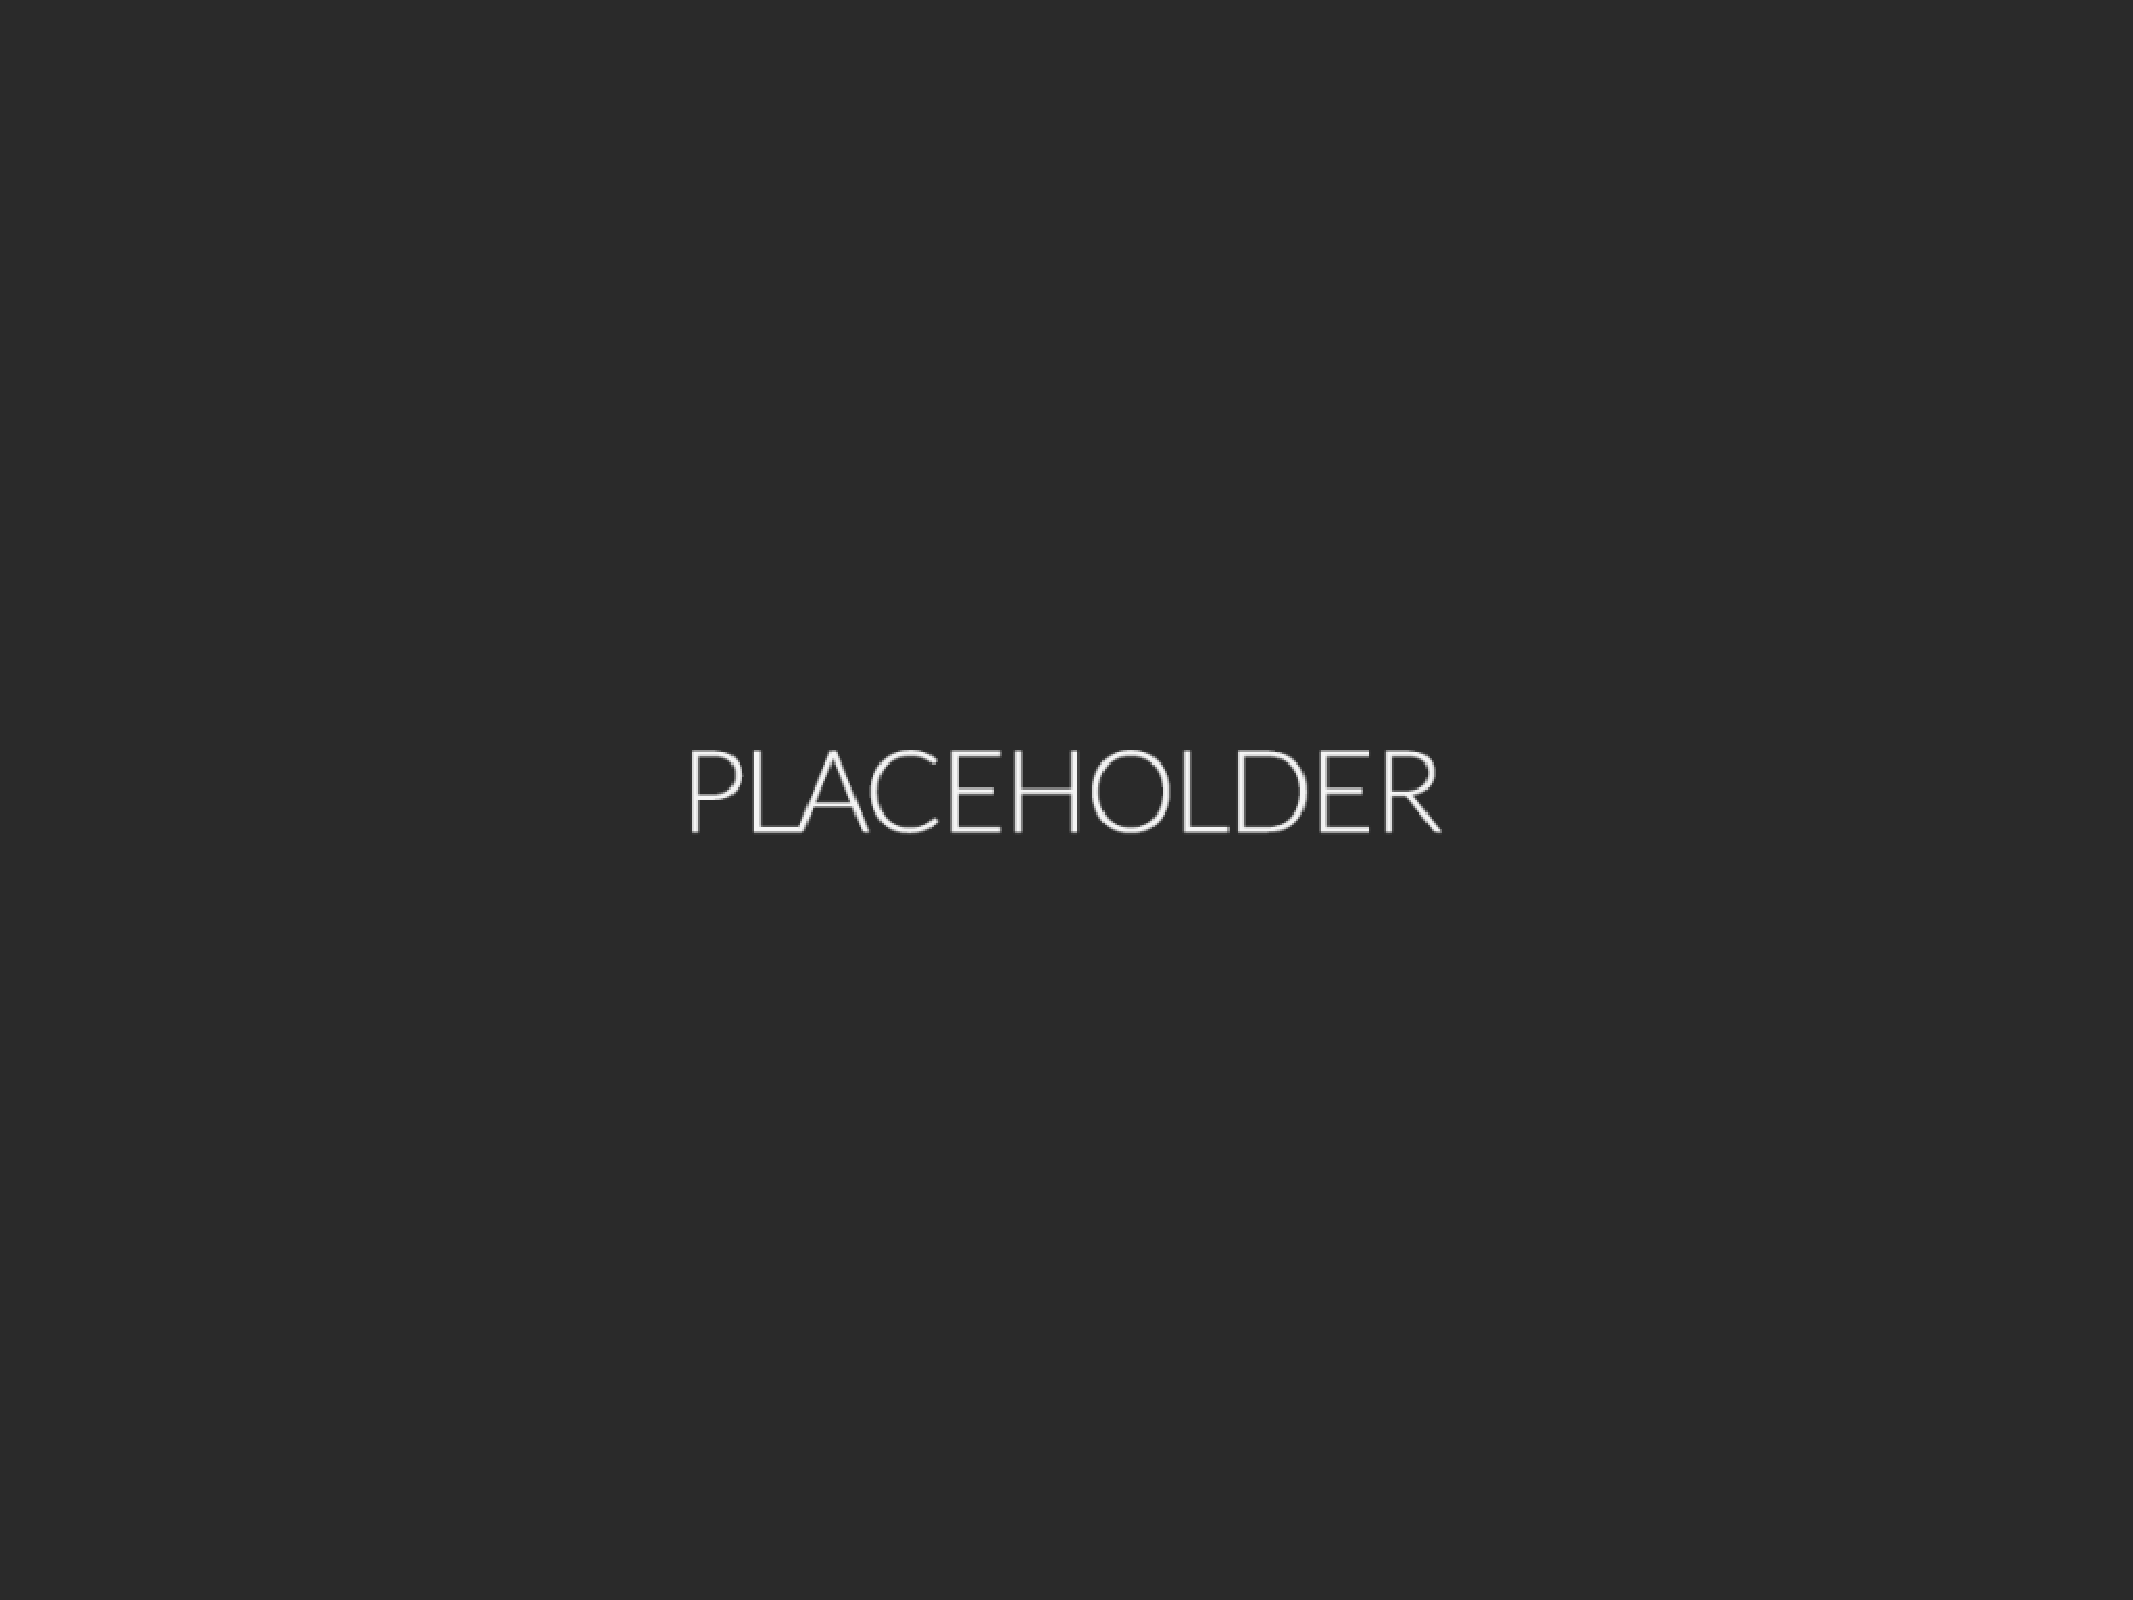
\includegraphics[width=0.5\columnwidth]{fig/placeholder.pdf}
    \caption{Caption goes here.}
\end{figure}


\renewcommand*{\MyPath}{./Chapters/ch6}
\renewcommand{\thechapter}{6}
\graphicspath{{\MyPath/}}

\chapter{Title} \label{sec:title}
Text.


\section{Title} \label{sec:section}
Text. \acrfull{asap}.


\section{Title} \label{sec:section}
Text.
%
\begin{figure}[H]
    \hypertarget{fig1}{}
    \centering
    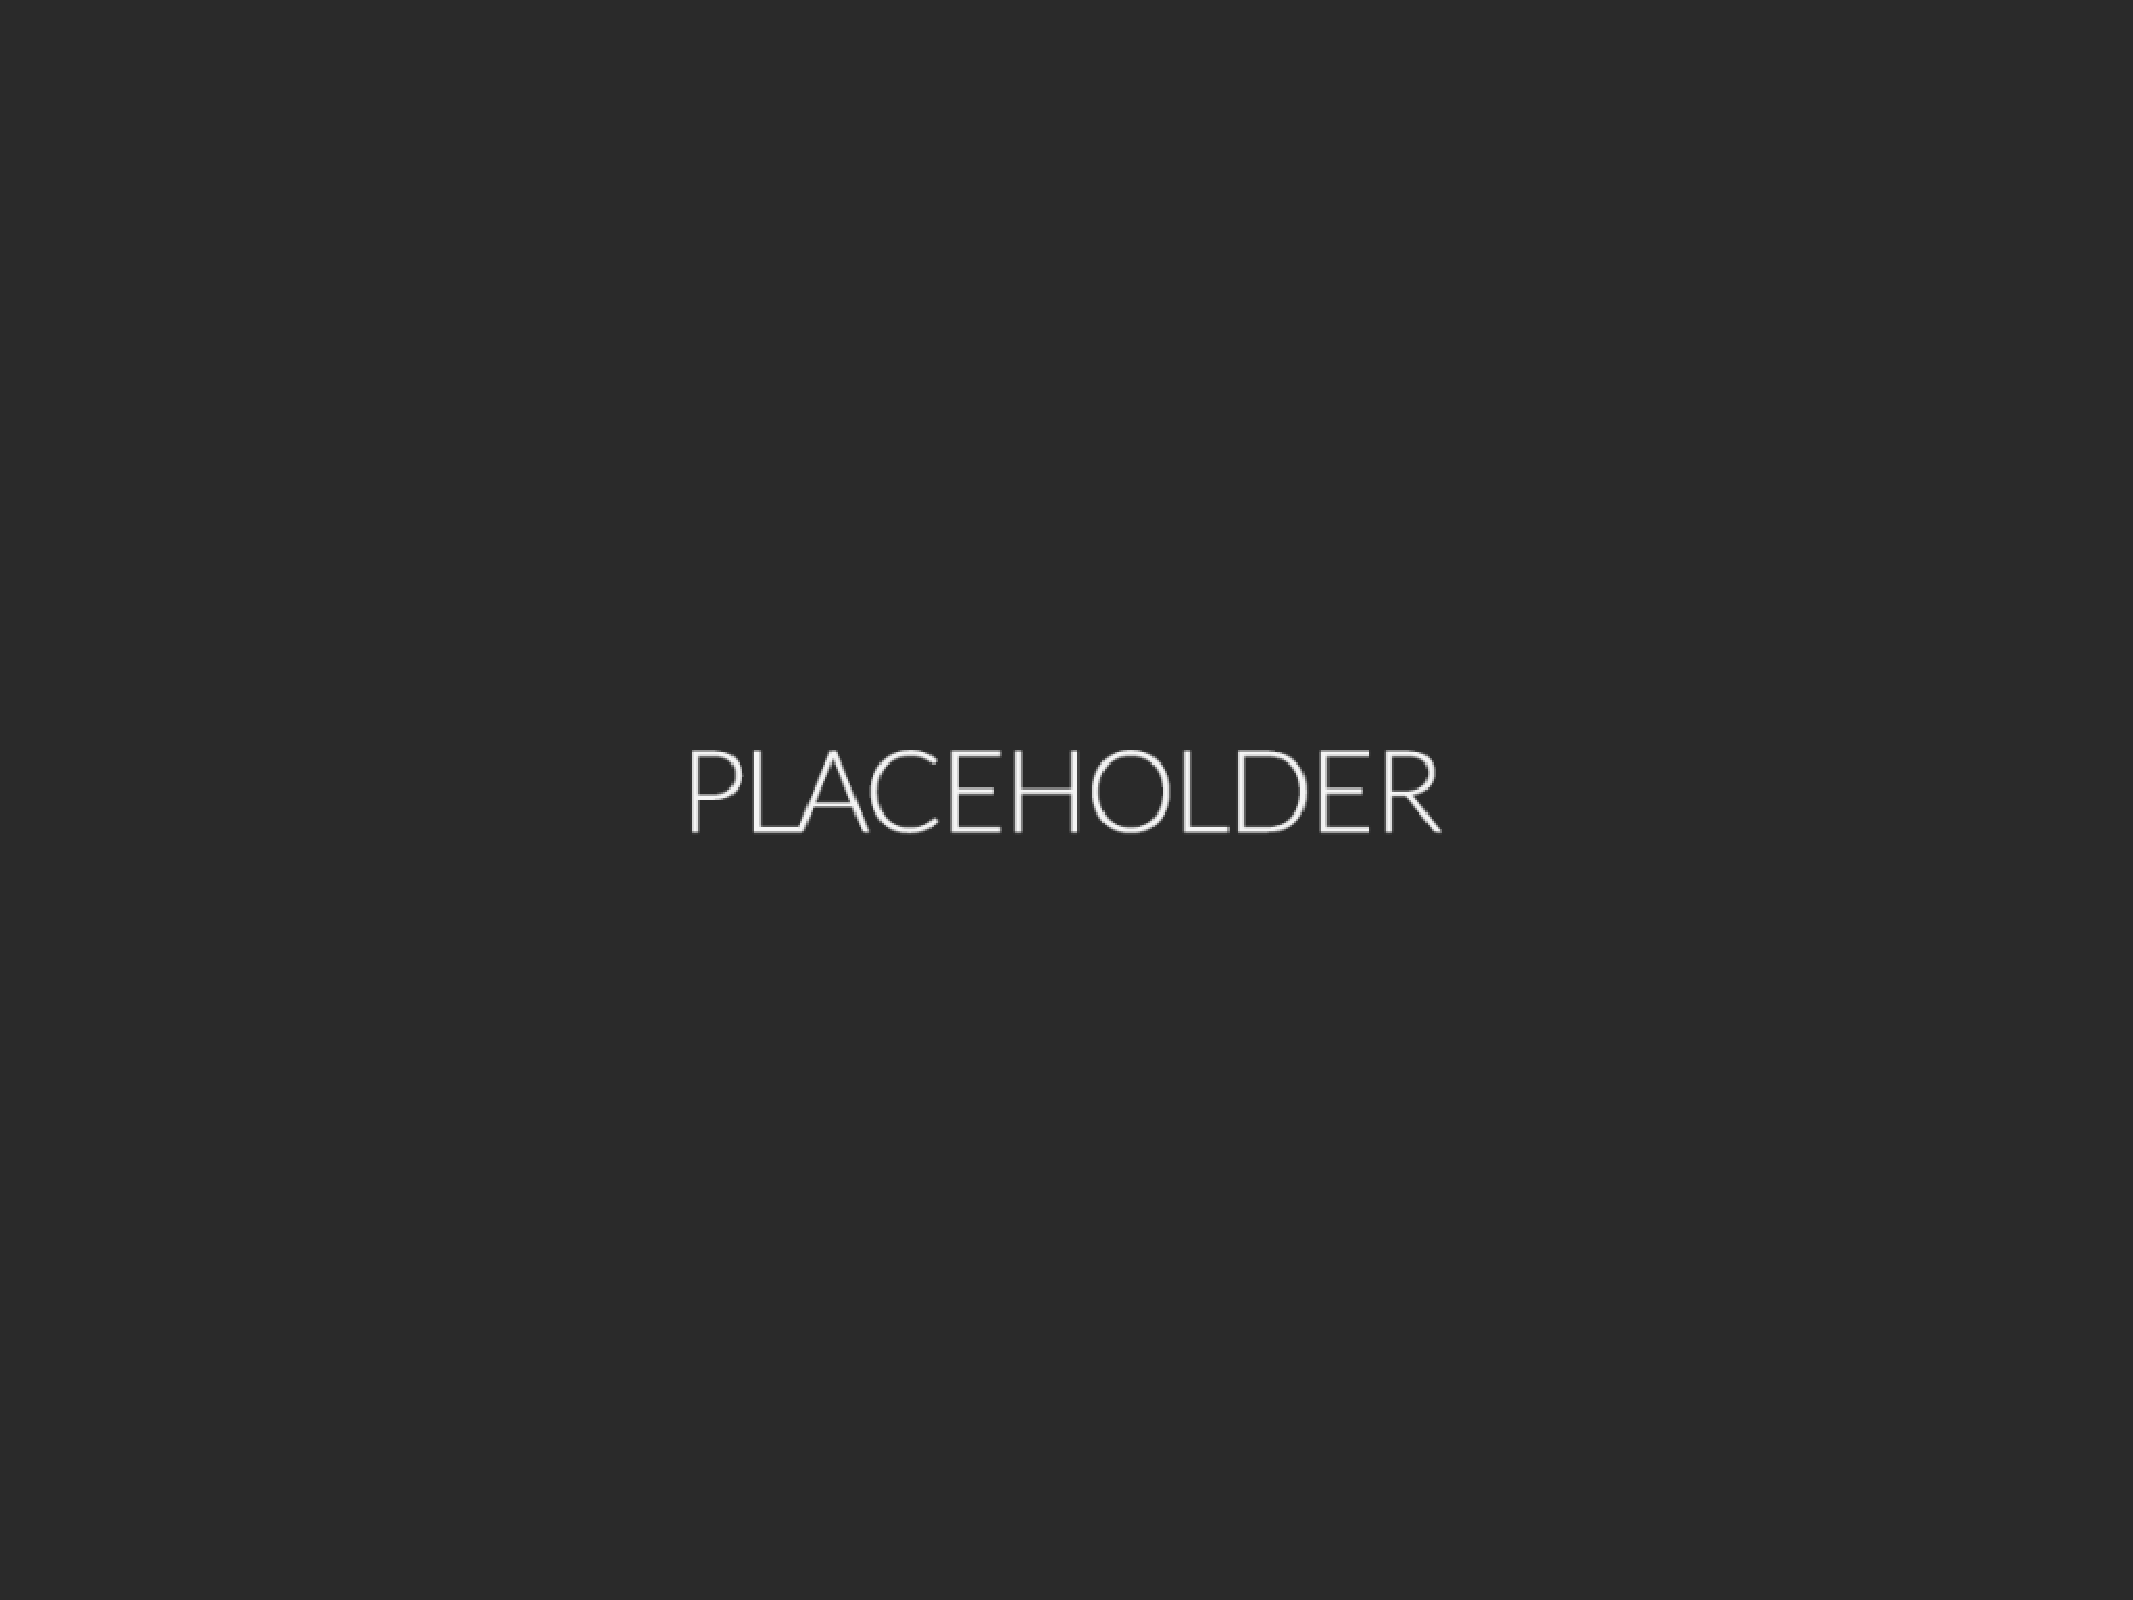
\includegraphics[width=0.5\columnwidth]{fig/placeholder.pdf}
    \caption{Caption goes here.}
\end{figure}
%
\begin{figure}[H]
    \hypertarget{fig2}{}
    \centering
    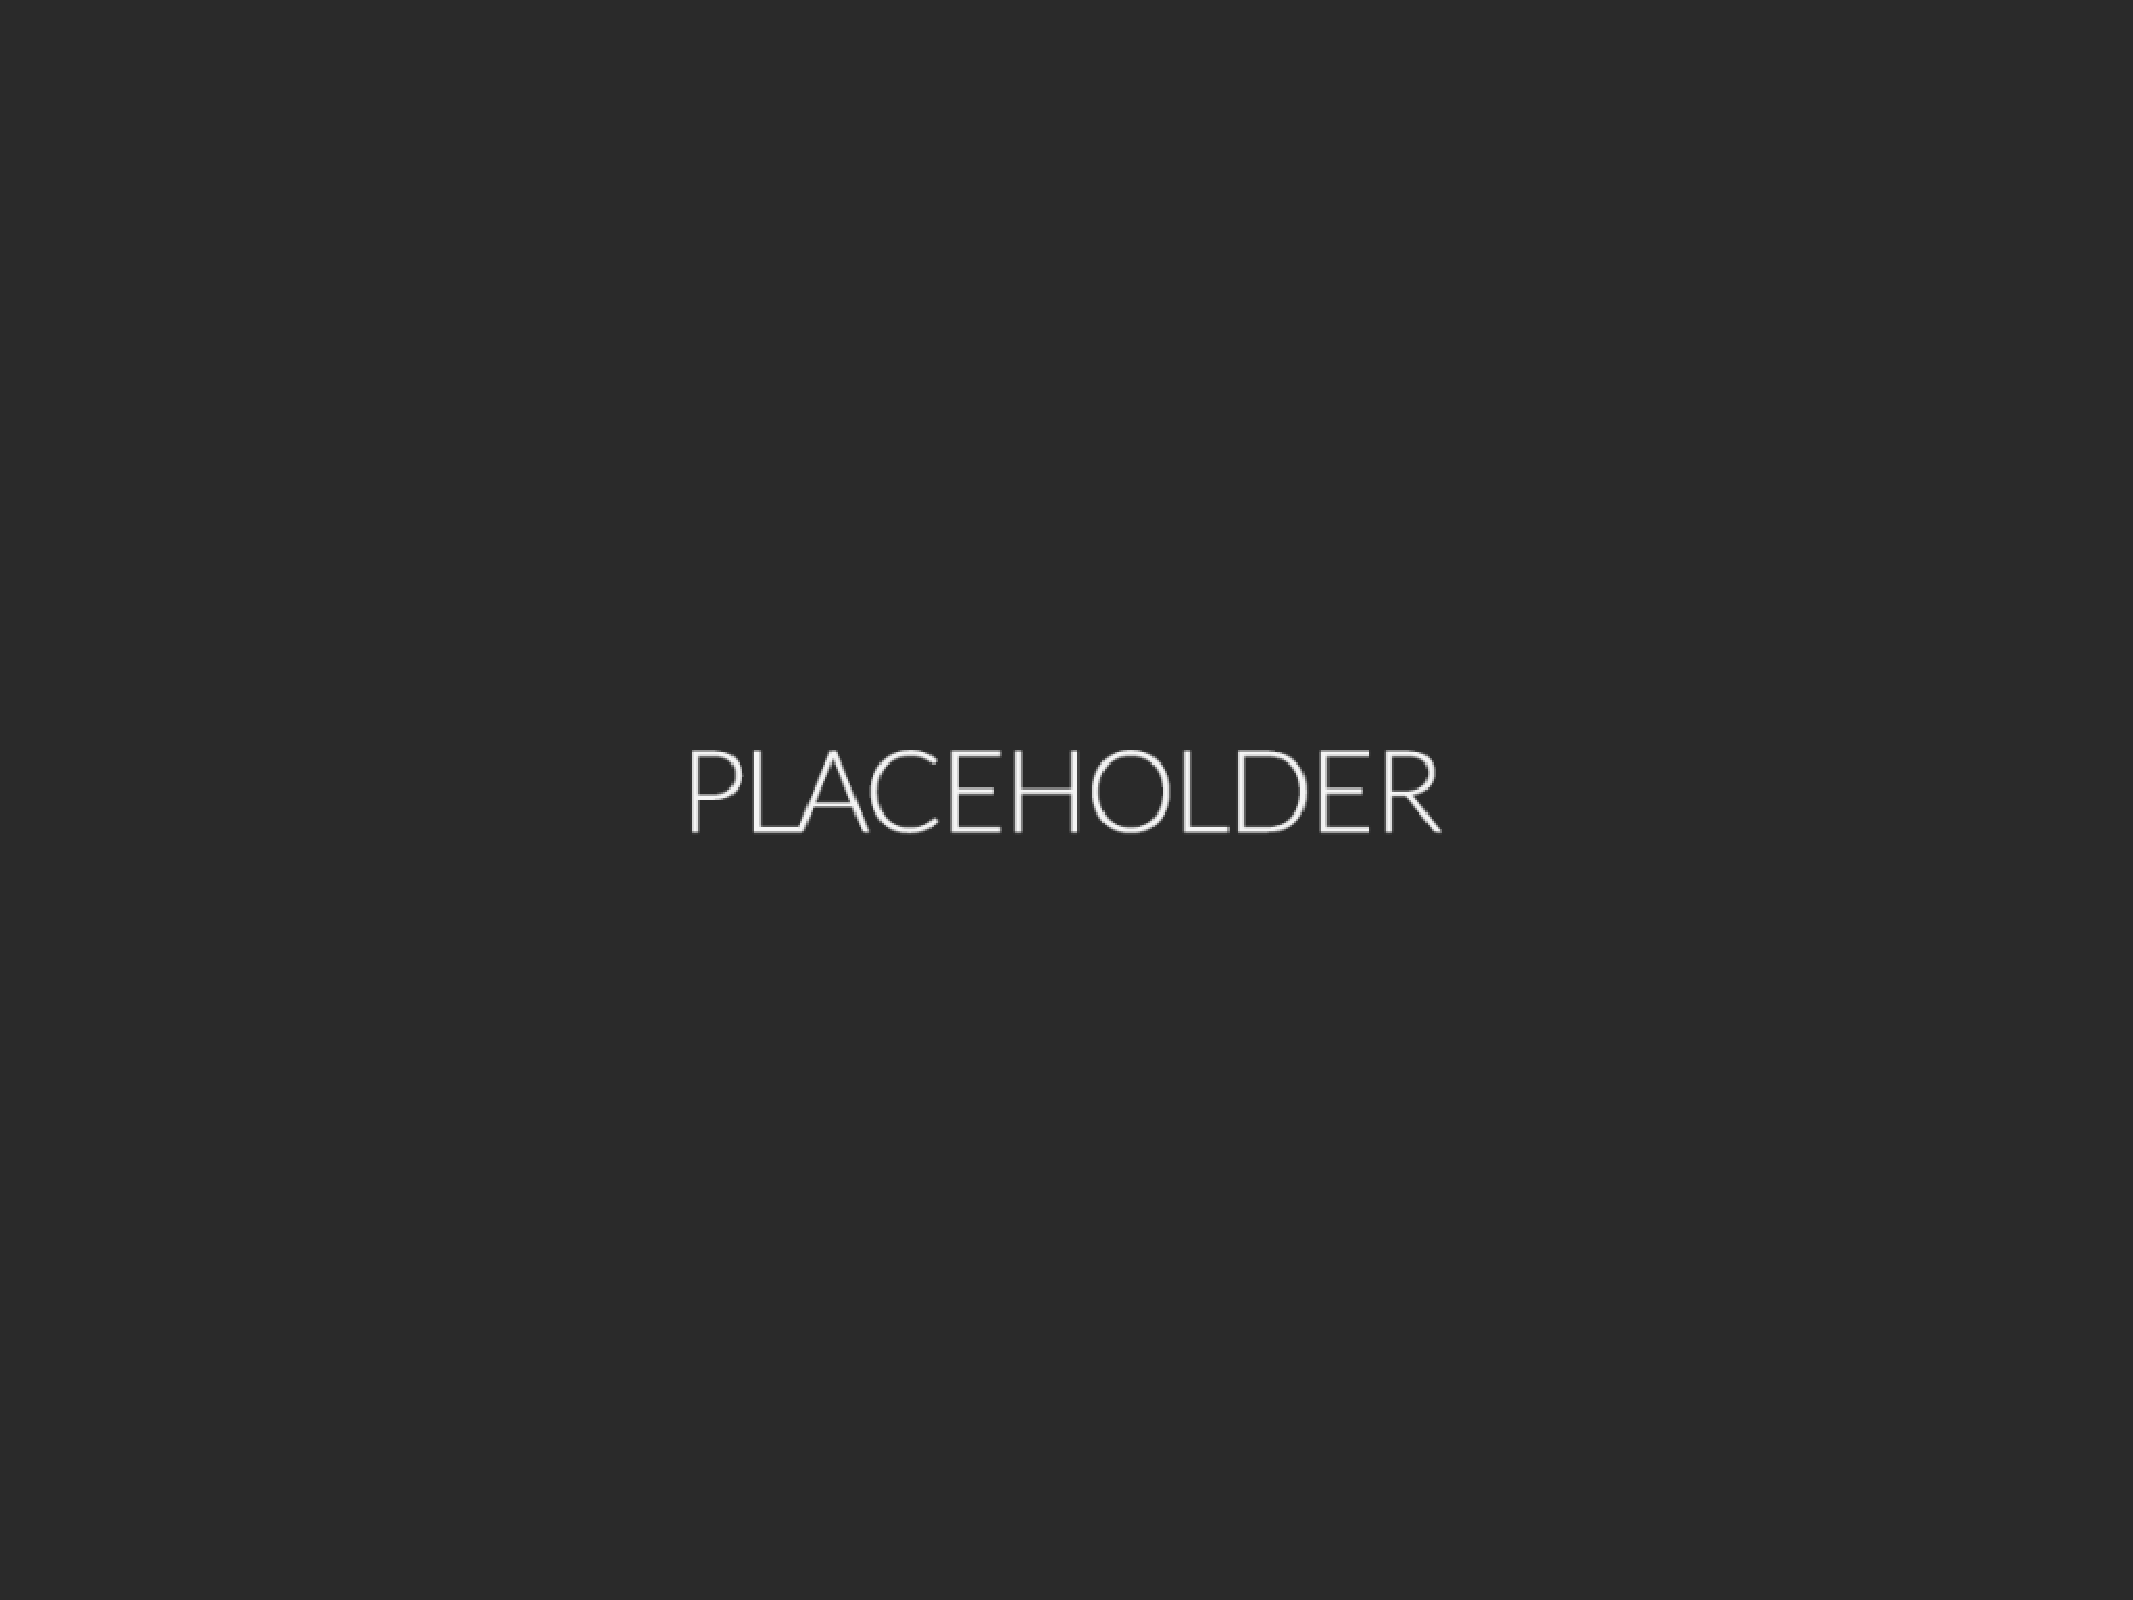
\includegraphics[width=0.5\columnwidth]{fig/placeholder.pdf}
    \caption{Caption goes here.}
\end{figure}


\renewcommand*{\MyPath}{./Chapters/ch6}
\renewcommand{\thechapter}{6}
\graphicspath{{\MyPath/}}

\chapter{Title} \label{sec:title}
Text.


\section{Title} \label{sec:section}
Text. \acrfull{asap}.


\section{Title} \label{sec:section}
Text.
%
\begin{figure}[H]
    \hypertarget{fig1}{}
    \centering
    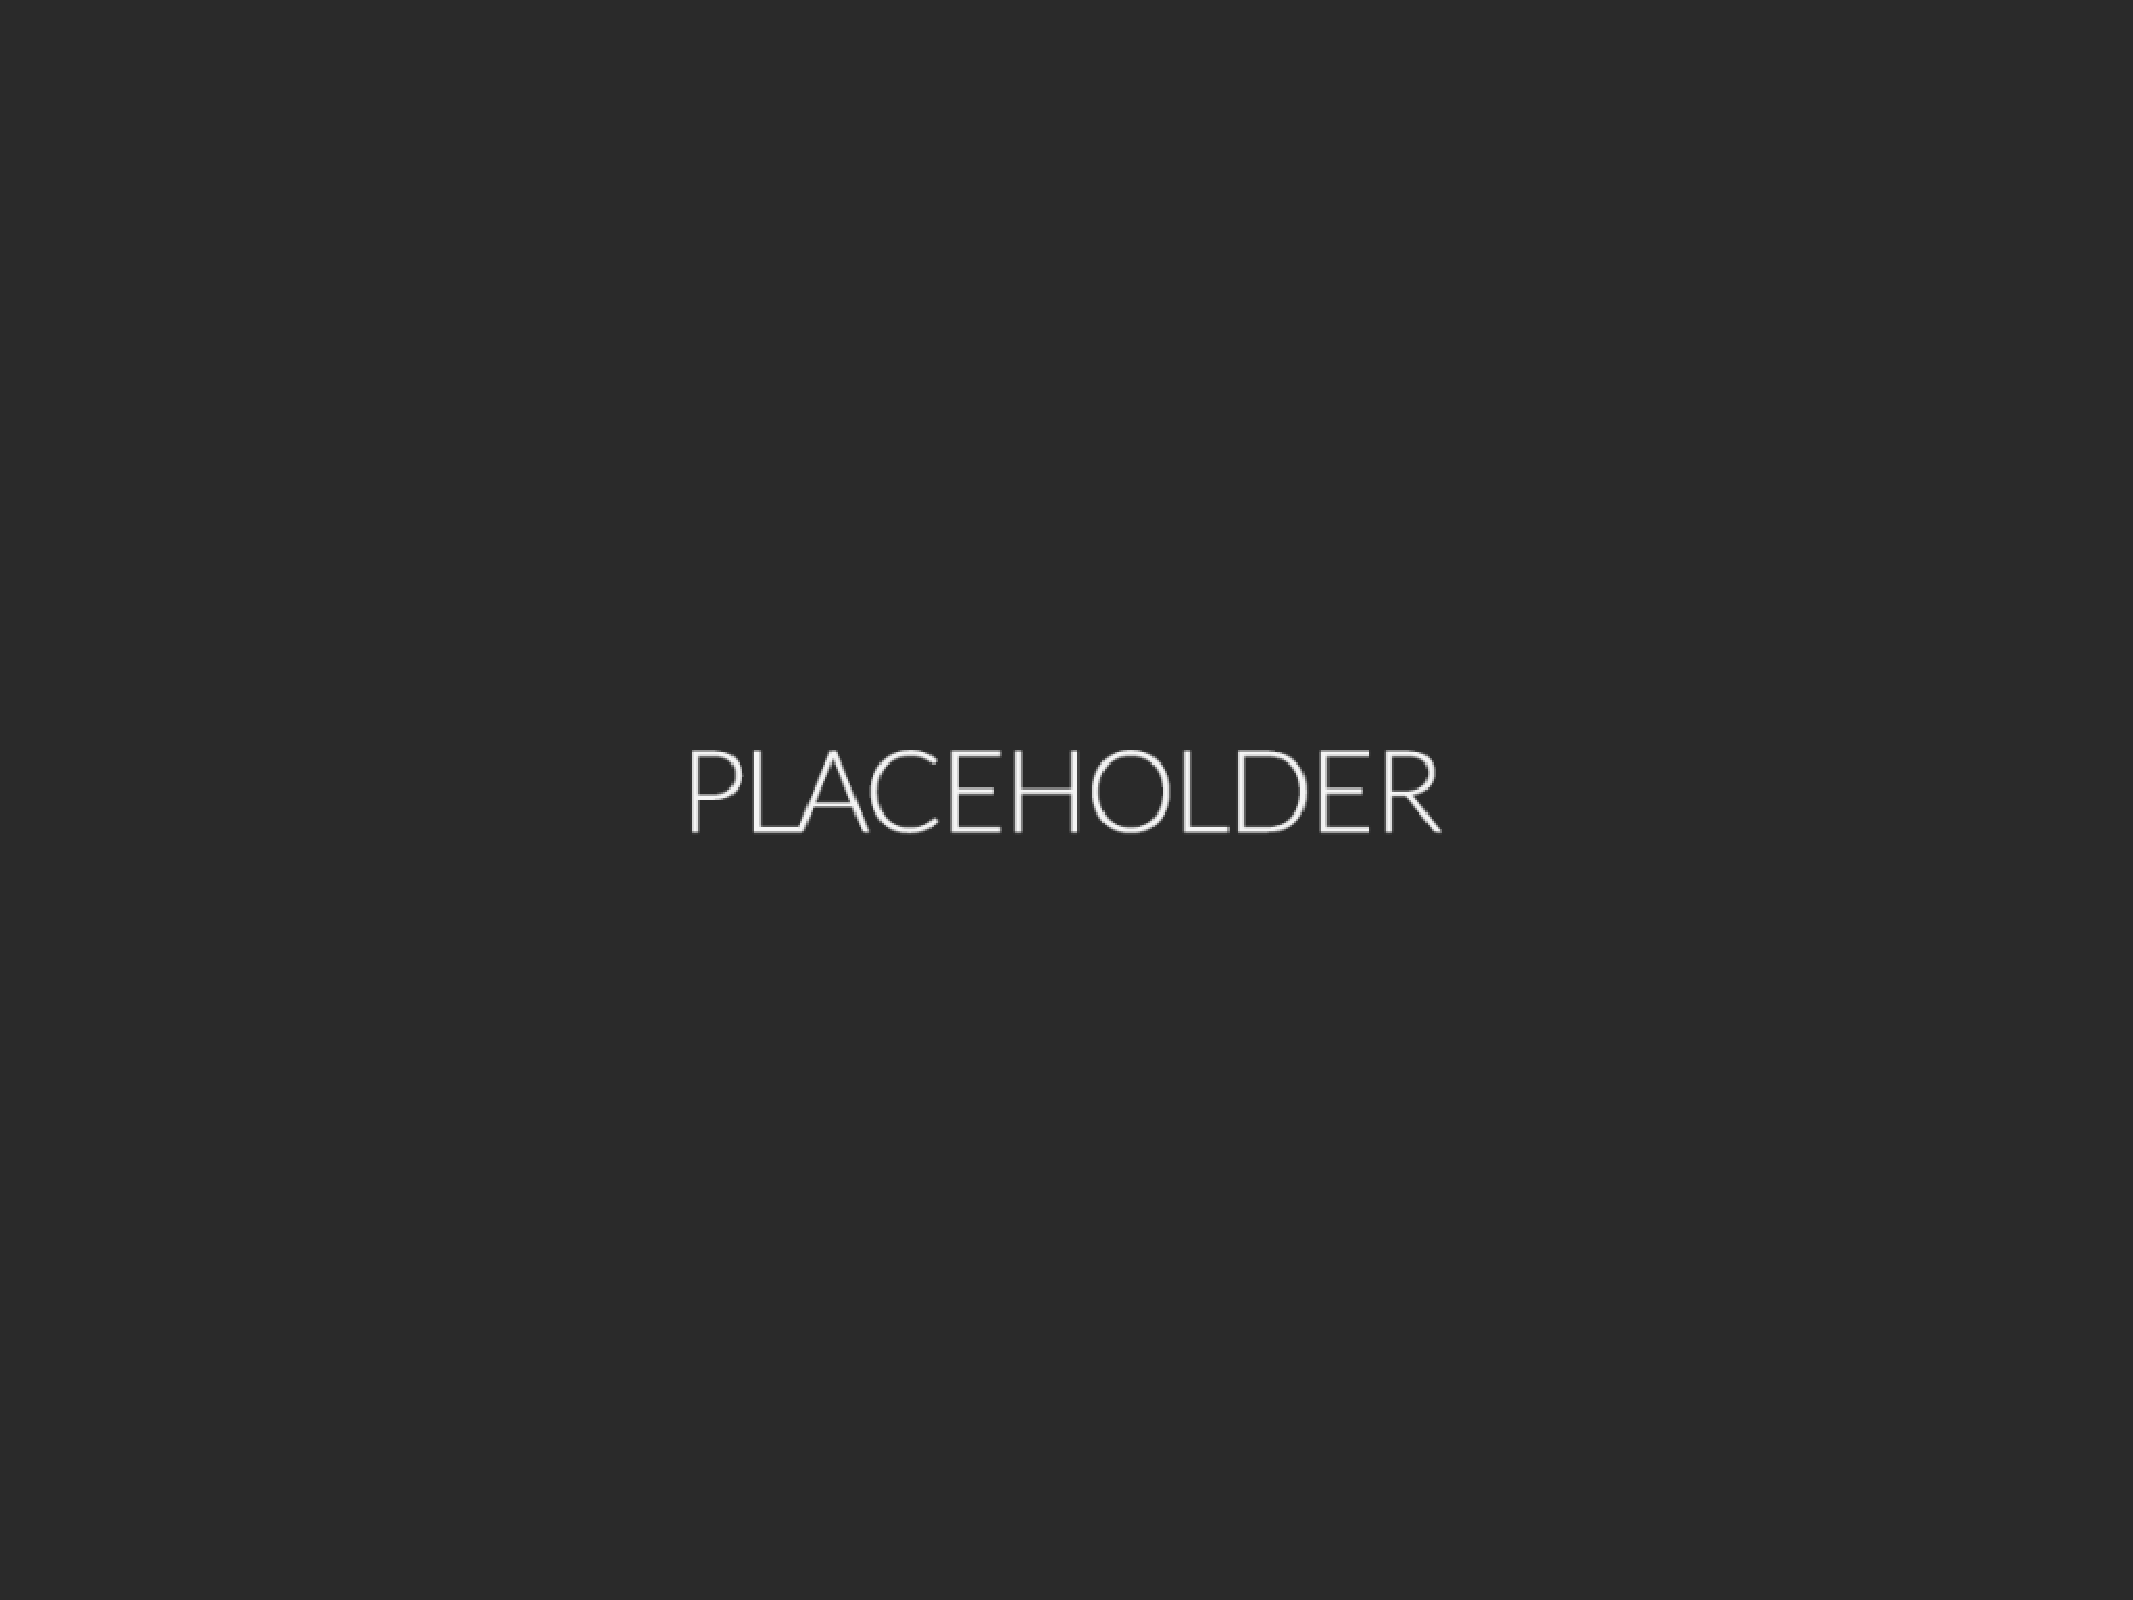
\includegraphics[width=0.5\columnwidth]{fig/placeholder.pdf}
    \caption{Caption goes here.}
\end{figure}
%
\begin{figure}[H]
    \hypertarget{fig2}{}
    \centering
    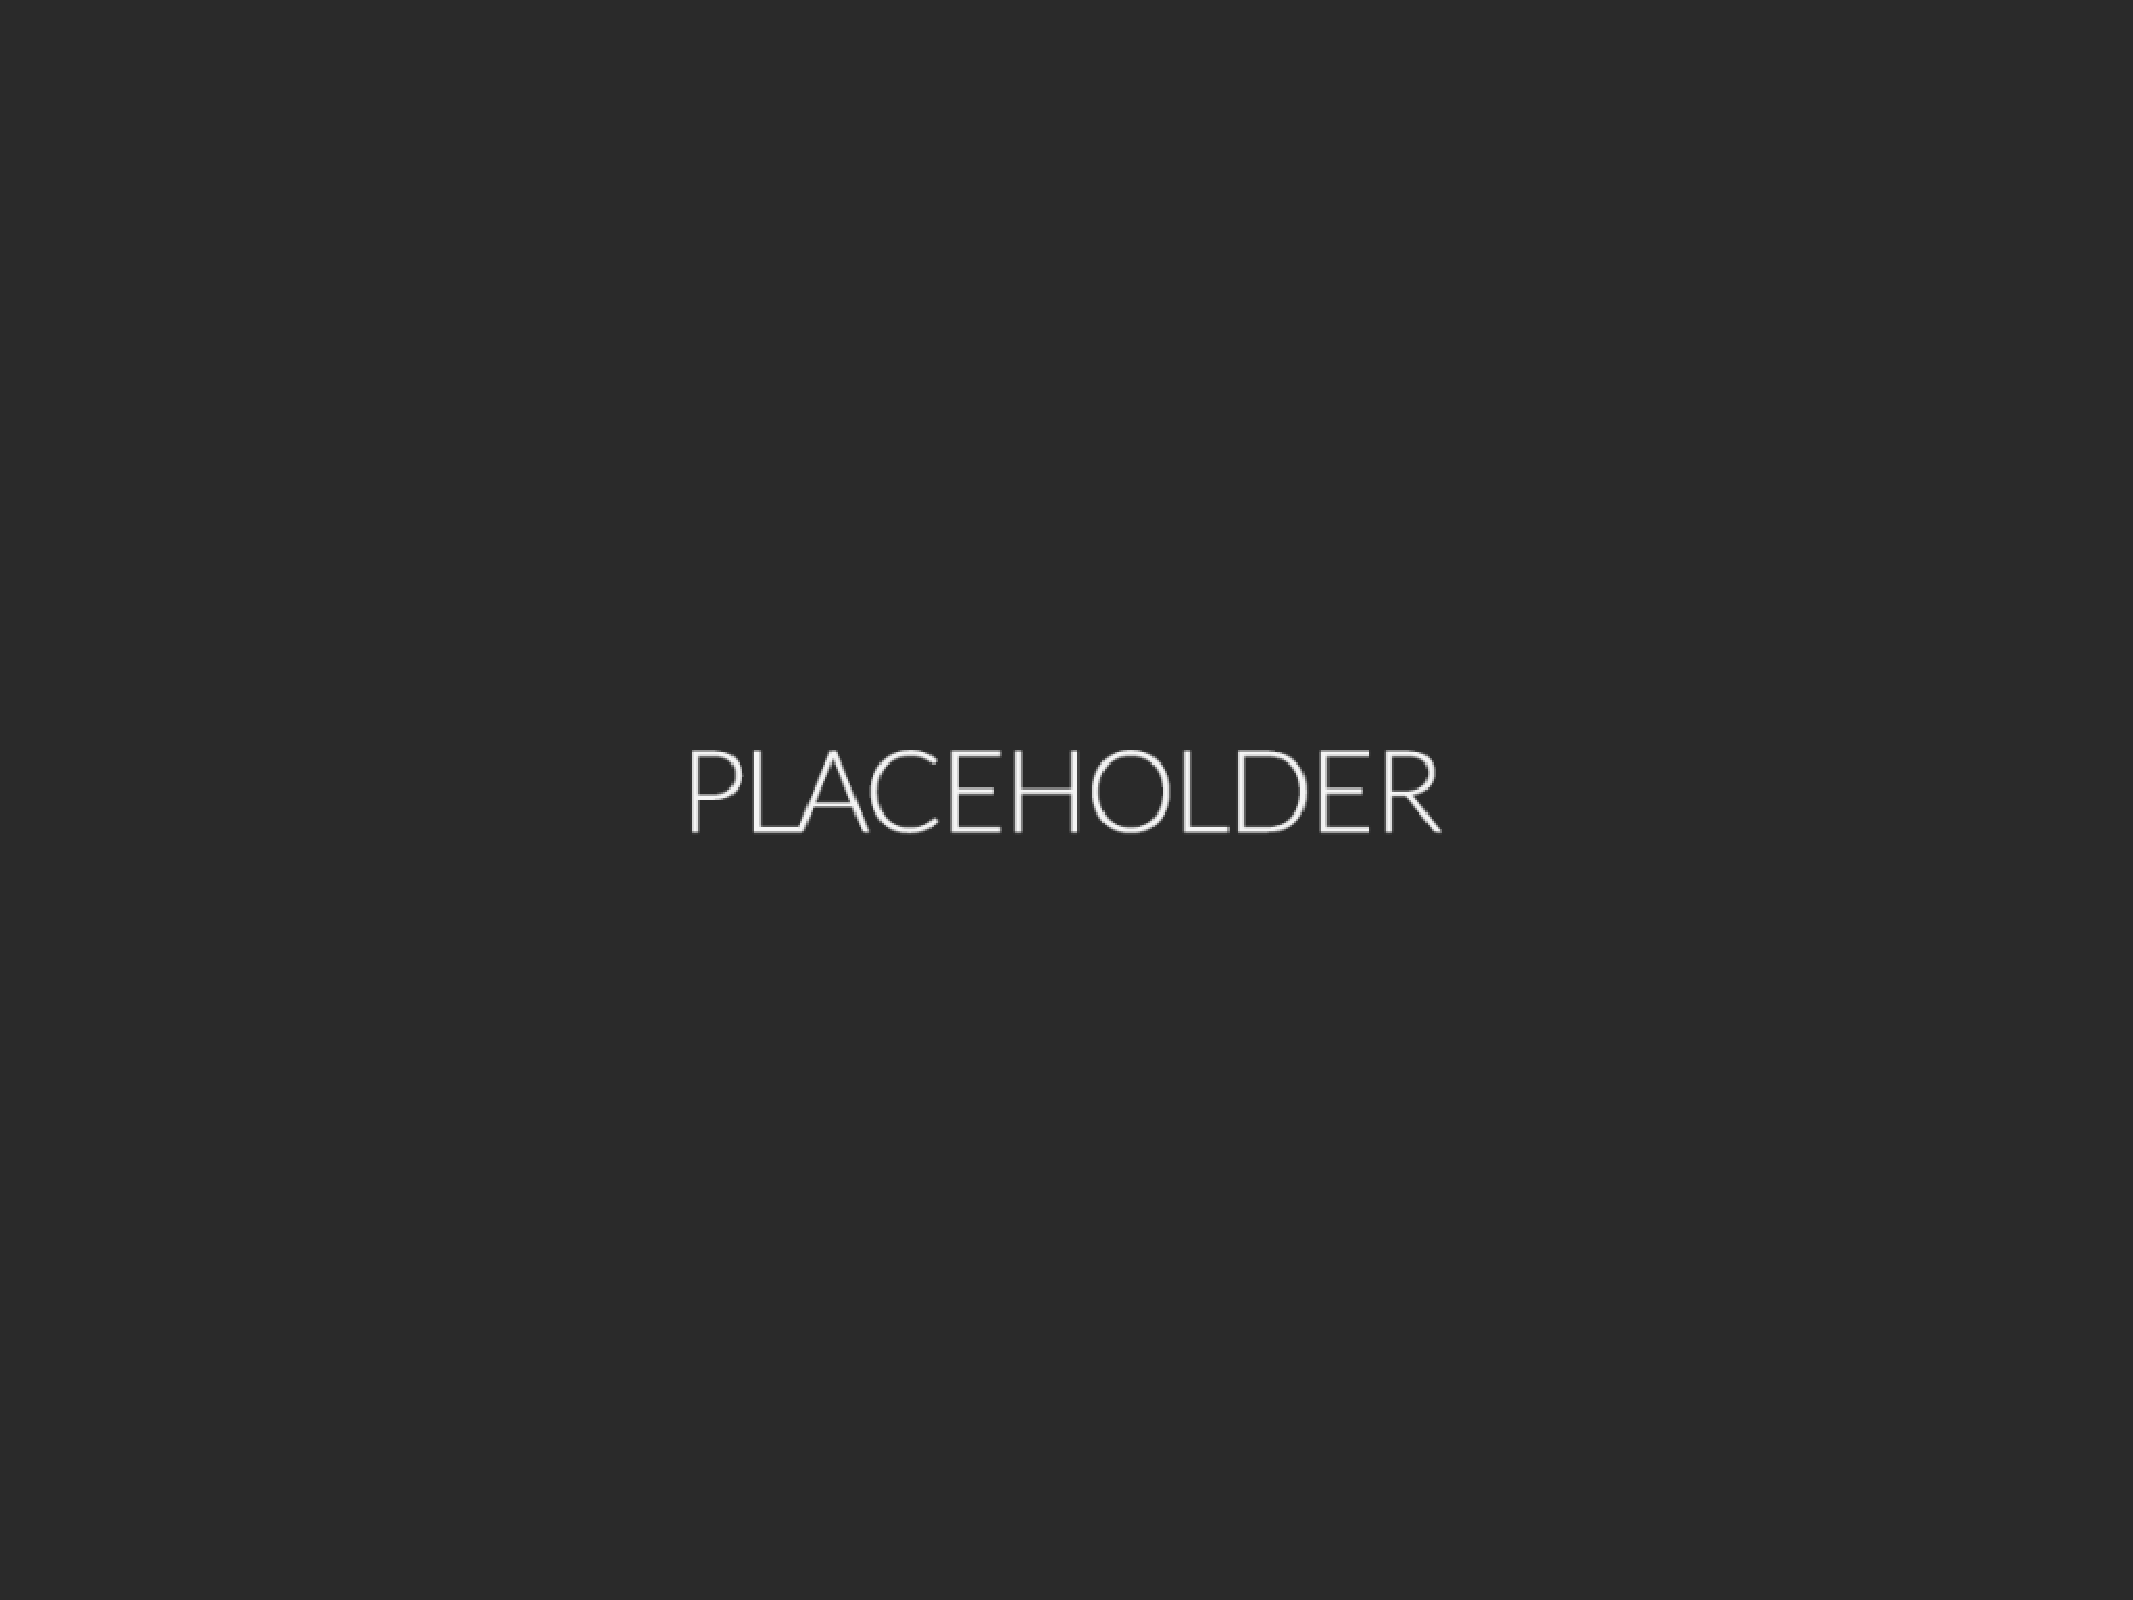
\includegraphics[width=0.5\columnwidth]{fig/placeholder.pdf}
    \caption{Caption goes here.}
\end{figure}



\begin{appendix}
	\renewcommand*{\MyPath}{./Chapters/ch6}
\renewcommand{\thechapter}{6}
\graphicspath{{\MyPath/}}

\chapter{Title} \label{sec:title}
Text.


\section{Title} \label{sec:section}
Text. \acrfull{asap}.


\section{Title} \label{sec:section}
Text.
%
\begin{figure}[H]
    \hypertarget{fig1}{}
    \centering
    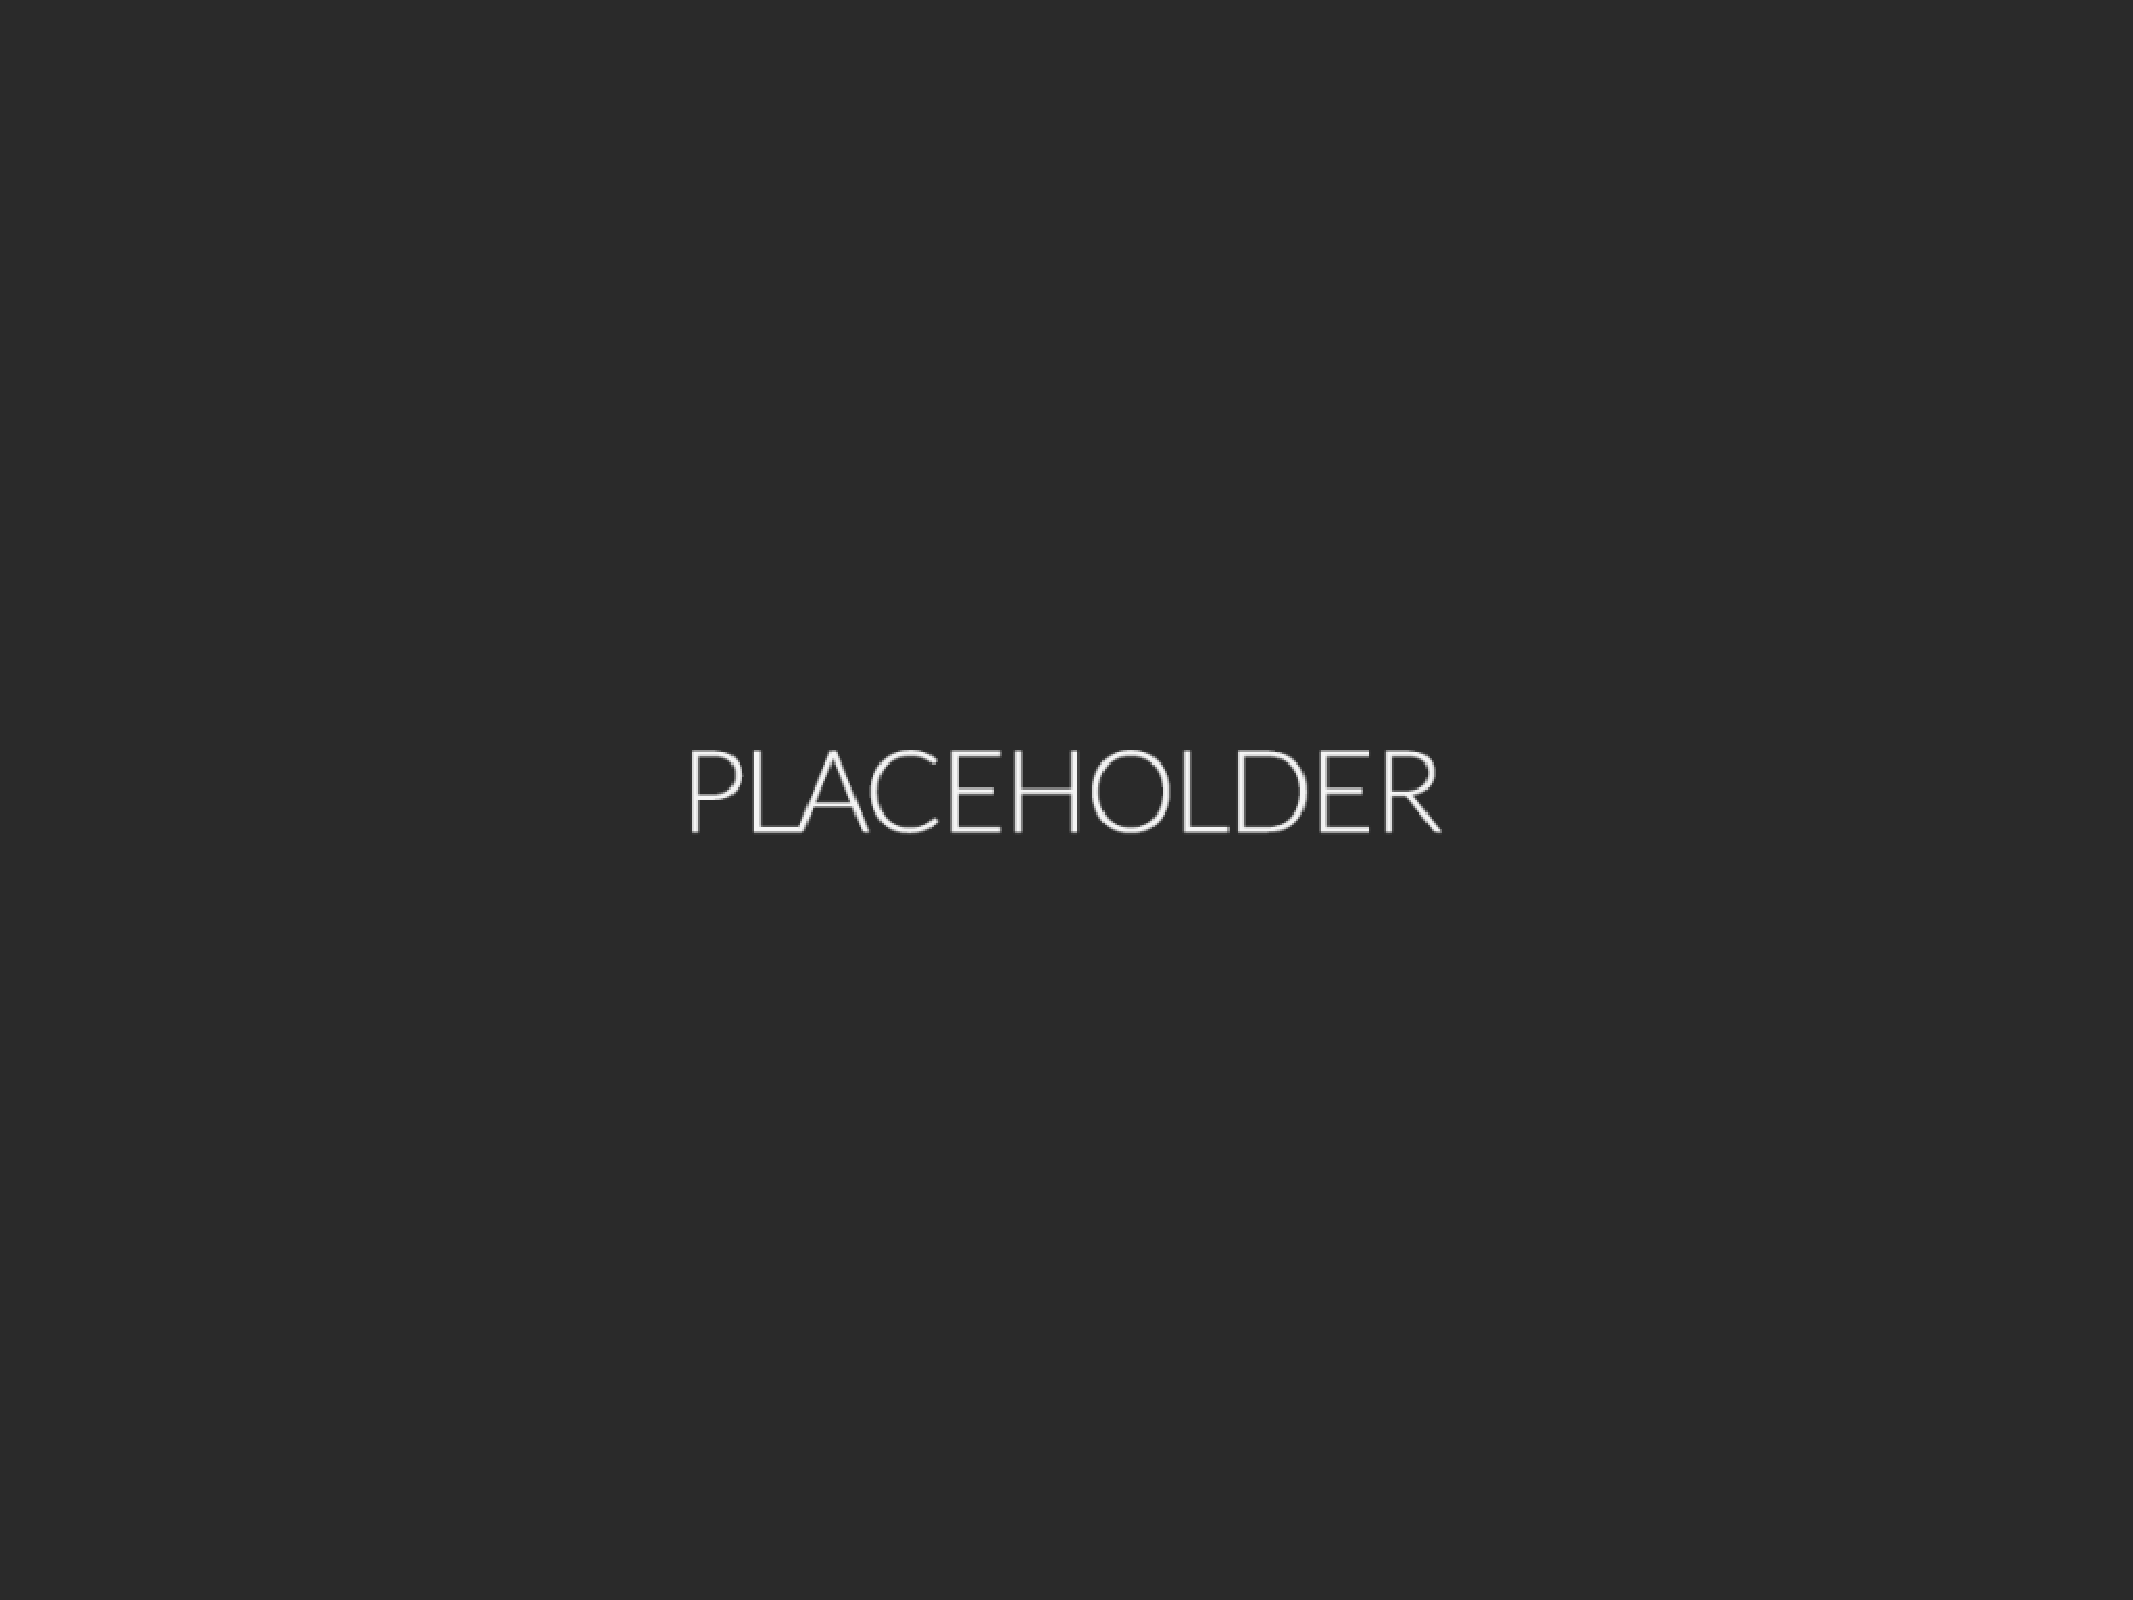
\includegraphics[width=0.5\columnwidth]{fig/placeholder.pdf}
    \caption{Caption goes here.}
\end{figure}
%
\begin{figure}[H]
    \hypertarget{fig2}{}
    \centering
    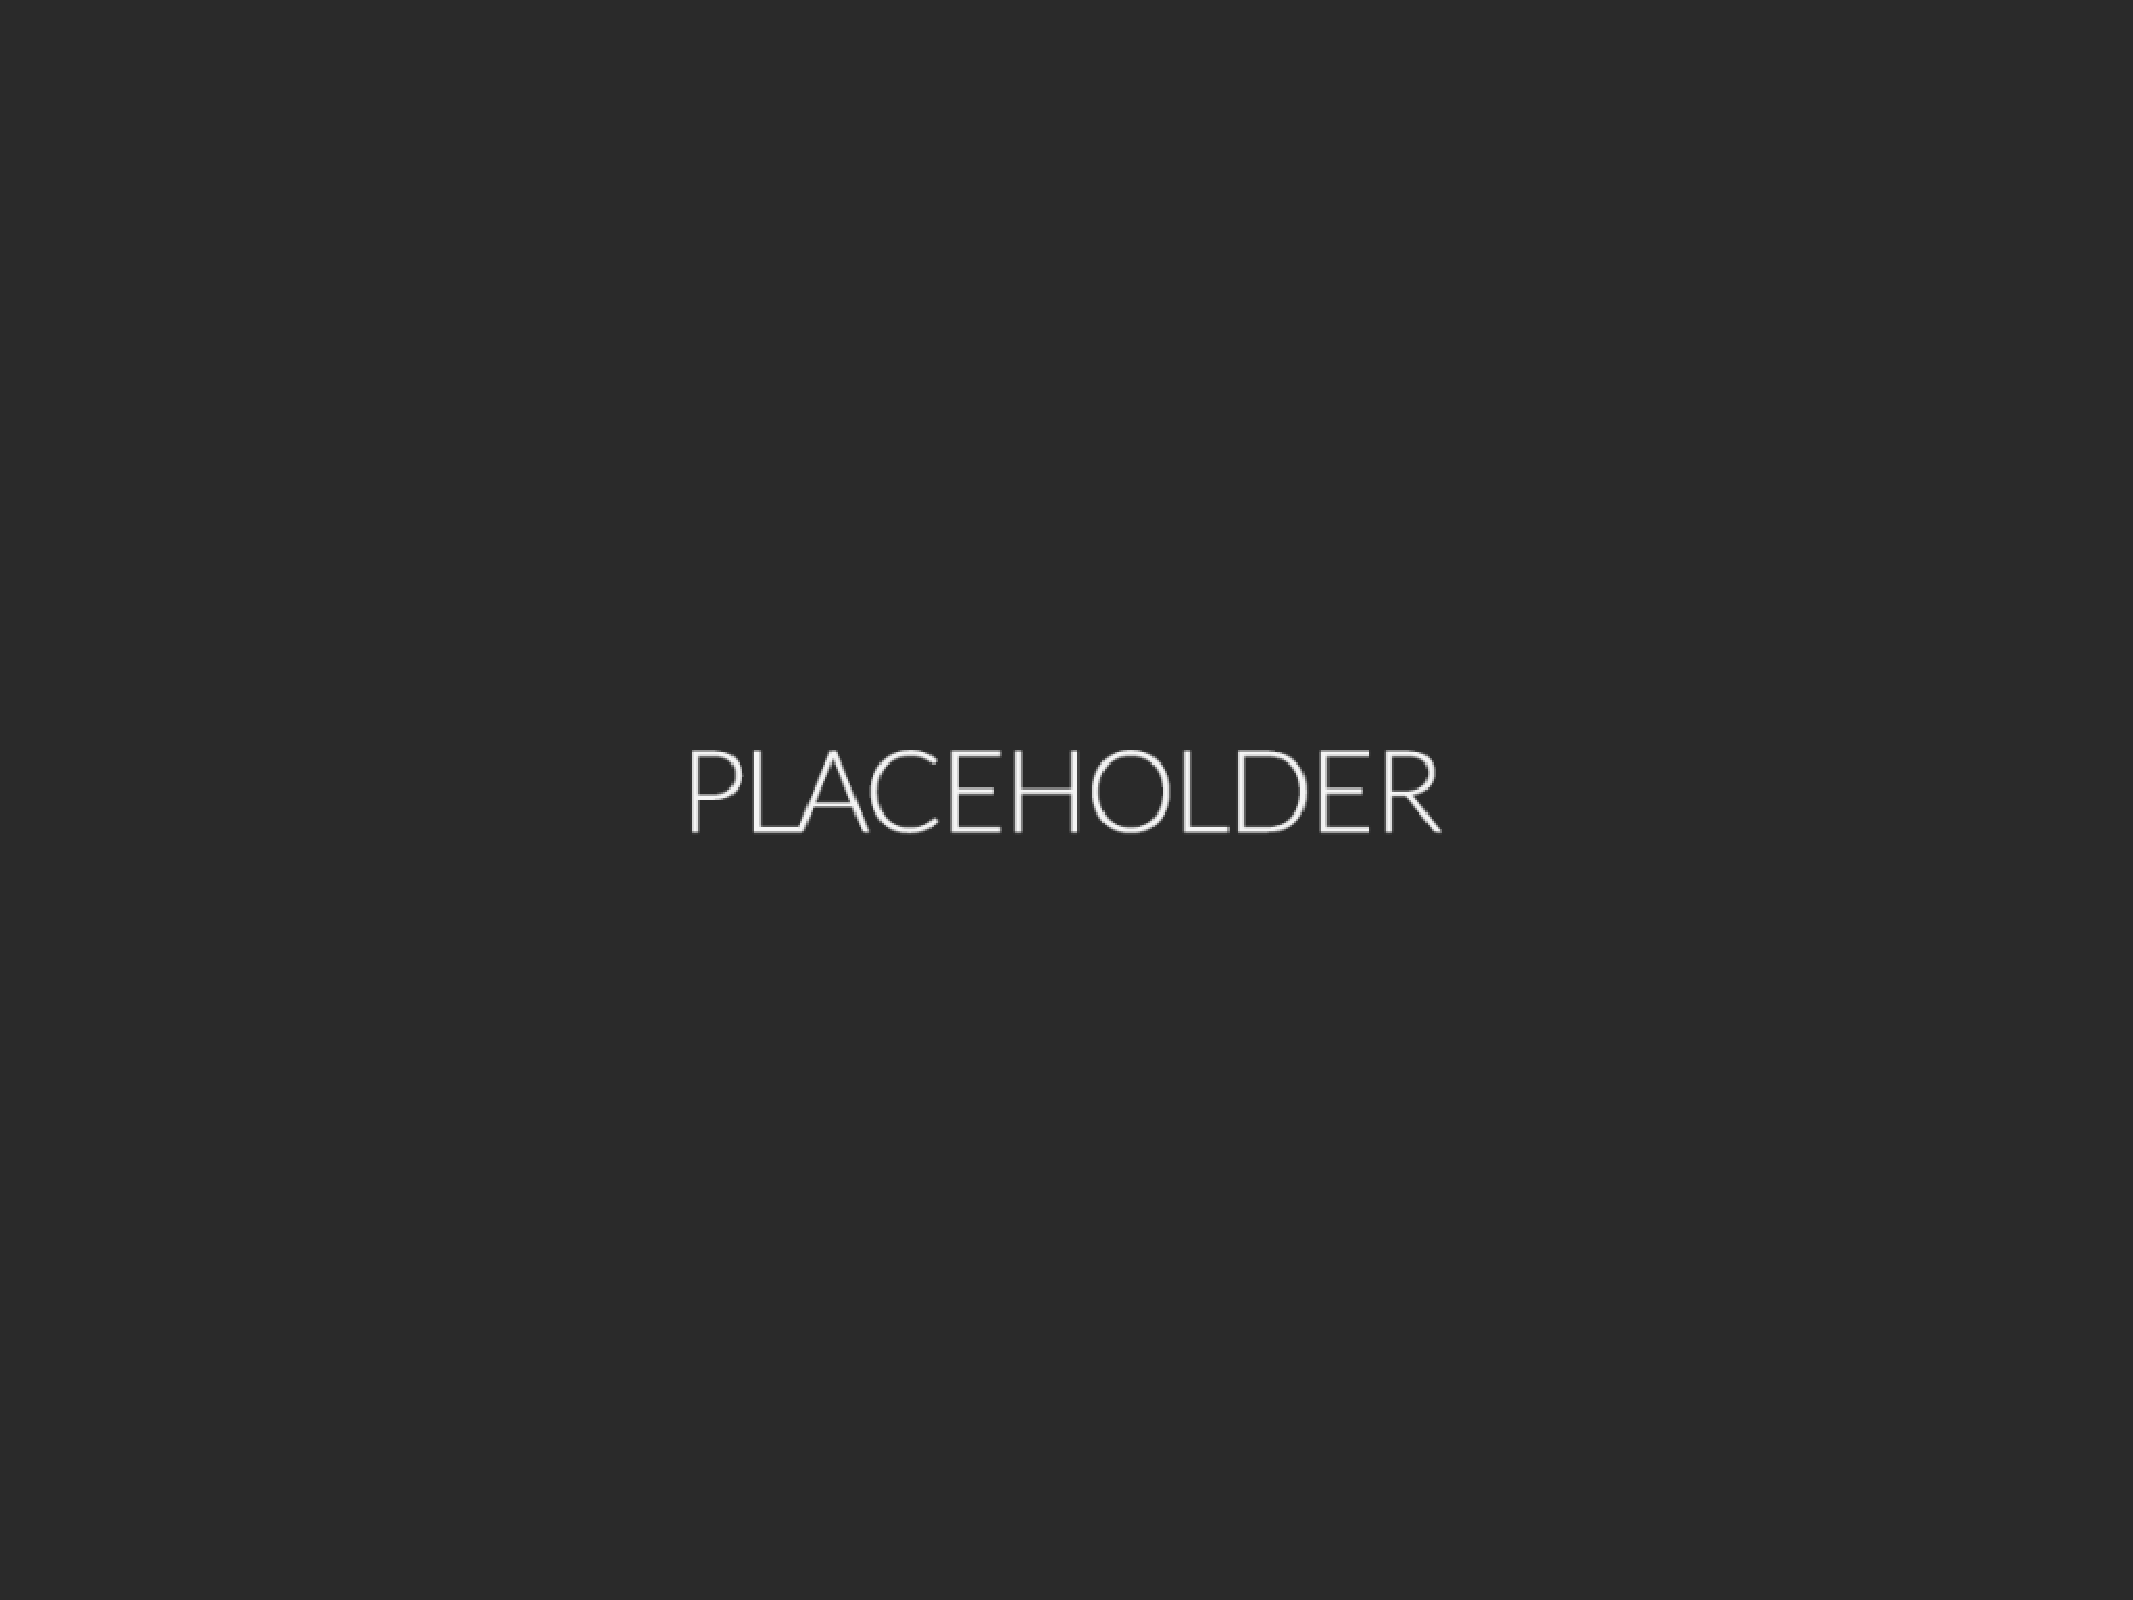
\includegraphics[width=0.5\columnwidth]{fig/placeholder.pdf}
    \caption{Caption goes here.}
\end{figure}


	\renewcommand*{\MyPath}{./Chapters/ch6}
\renewcommand{\thechapter}{6}
\graphicspath{{\MyPath/}}

\chapter{Title} \label{sec:title}
Text.


\section{Title} \label{sec:section}
Text. \acrfull{asap}.


\section{Title} \label{sec:section}
Text.
%
\begin{figure}[H]
    \hypertarget{fig1}{}
    \centering
    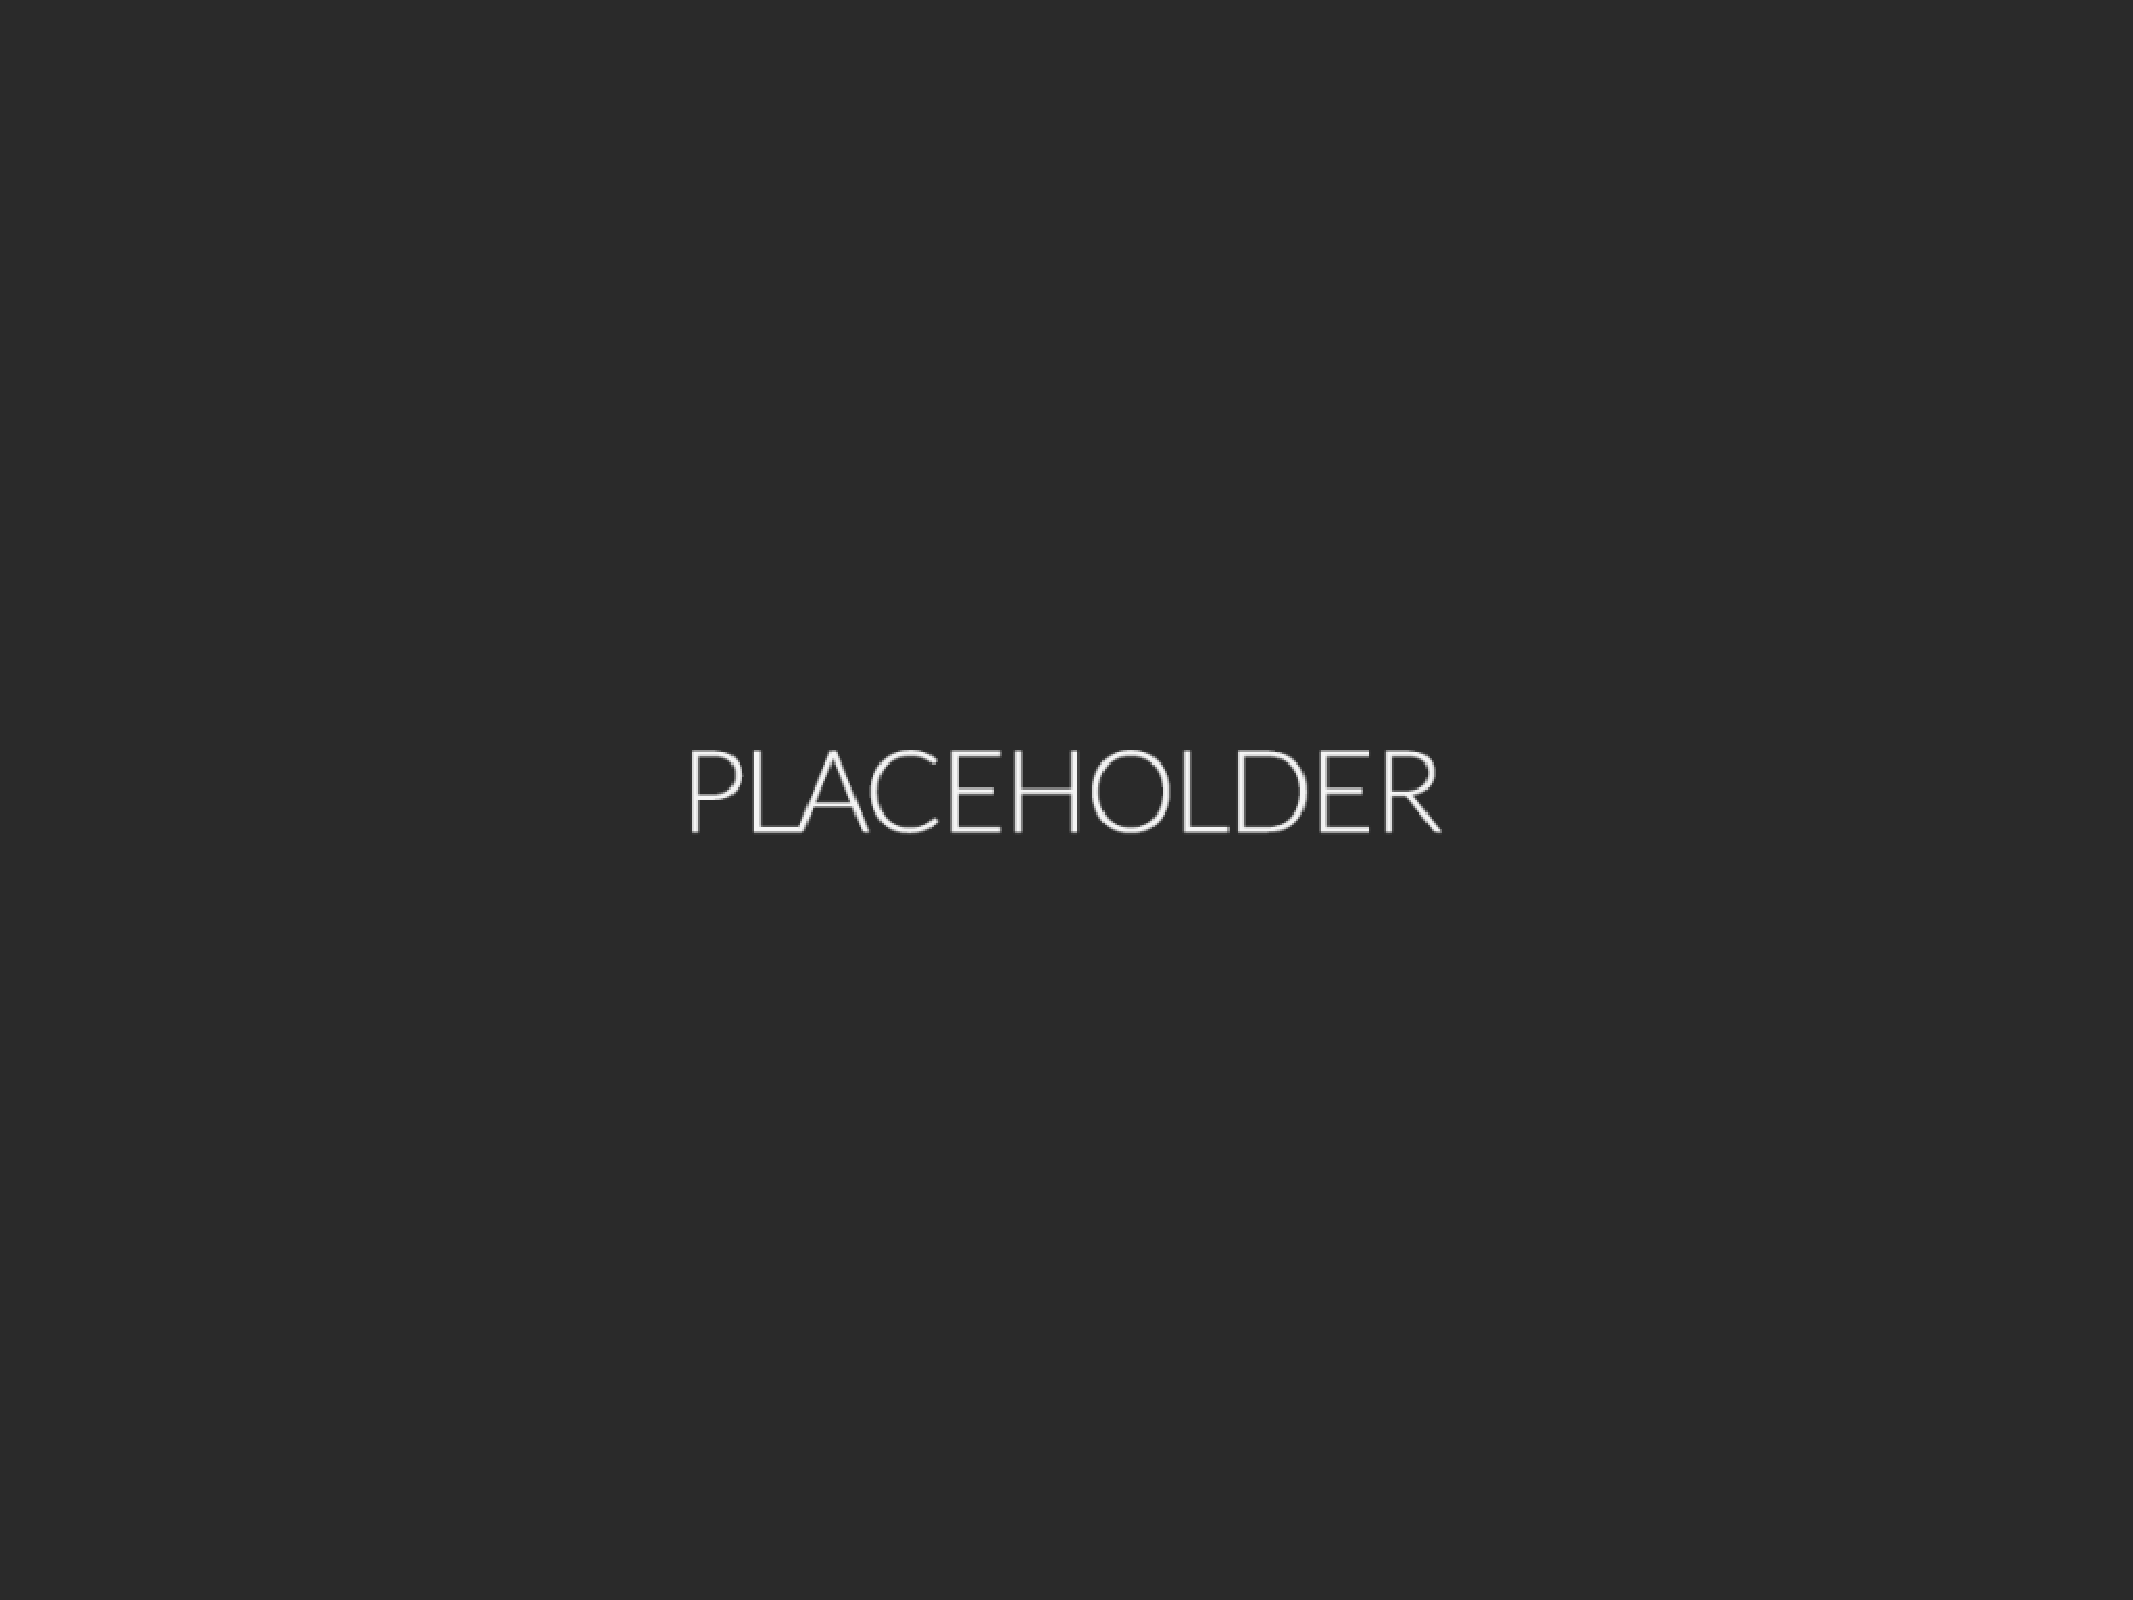
\includegraphics[width=0.5\columnwidth]{fig/placeholder.pdf}
    \caption{Caption goes here.}
\end{figure}
%
\begin{figure}[H]
    \hypertarget{fig2}{}
    \centering
    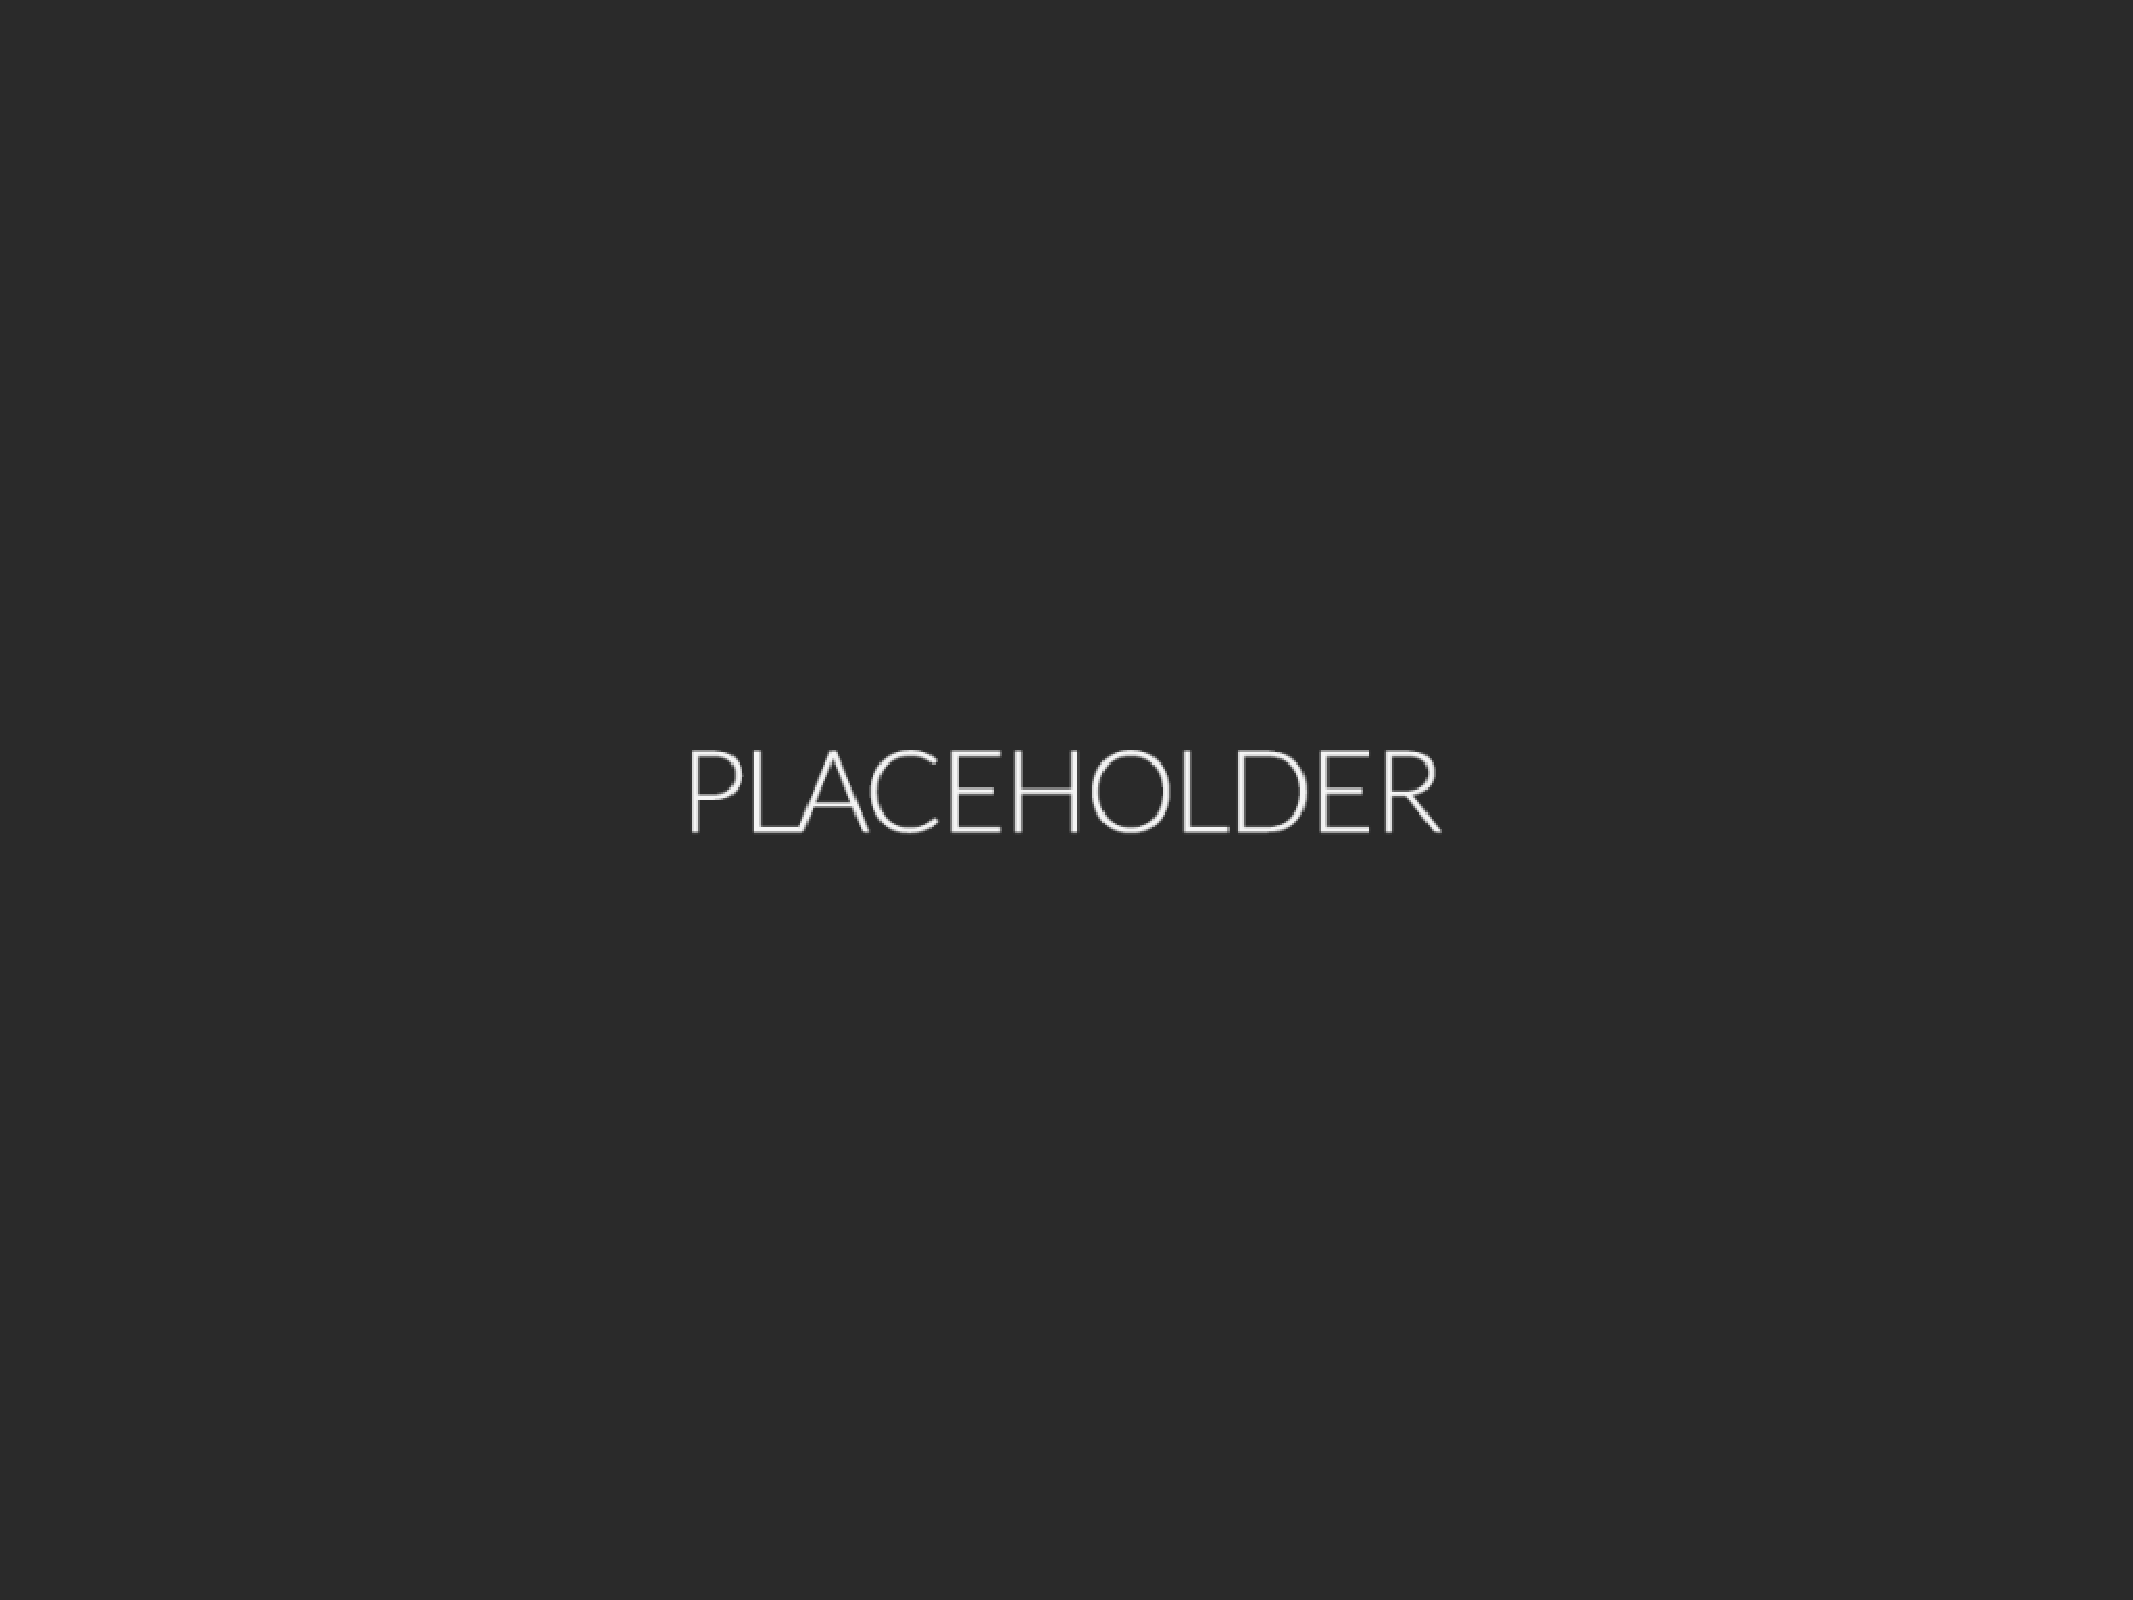
\includegraphics[width=0.5\columnwidth]{fig/placeholder.pdf}
    \caption{Caption goes here.}
\end{figure}


\end{appendix}

\printbibliography

\end{document}
